\documentclass[12pt,a4paper,openany,UKenglish]{scrreprt}
\usepackage[hcentering, textwidth=17cm, top=2.5cm, bottom=2.5cm]{geometry}
\usepackage[colorlinks=true,linkcolor=black,urlcolor=purple,citecolor=blue,anchorcolor=blue]{hyperref}
\usepackage[T1]{fontenc}
\usepackage[utf8]{inputenc}
\usepackage{graphicx, wrapfig}
\usepackage[x11names]{xcolor}
\usepackage[UKenglish]{babel}
\usepackage{amsmath}
\usepackage{amssymb}
\usepackage{pgfgantt}
\usepackage{csquotes}
\usepackage{lmodern}
\usepackage{multirow}
\usepackage{enumitem}
\usepackage{caption}
\usepackage{url}
\usepackage{float}
\usepackage{scrhack}

\newcommand{\bib}[1]{$^\text{\cite{#1}}$}

\begin{document}
\begin{titlepage}
	\centering
	\begin{figure}
		\begin{minipage}{0.5\textwidth}
			\begin{flushleft}
				
\includegraphics[width=.7\linewidth]{../Images/Logo_UTT.png}
			\end{flushleft}
		\end{minipage}\hfill
		\begin{minipage}{0.5\textwidth}
			\begin{flushright}
				
\includegraphics[width=.7\linewidth]{../Images/ifth_retina.png}
			\end{flushright}
		\end{minipage}
	\end{figure}
	\phantom{test}\\
	\par\vspace{4cm}
	{\Large\bfseries Morphotype of the human body in the textile industry: a clustering approach.\par}
	\vspace{4cm}
	Steve de Rose\\
	\vspace{4cm}
	\textit{Supervised by :}\\
	\small\href{mailto:frederic.bertrand@utt.fr}{Frédéric Bertrand (UTT)}\\
	\small\href{mailto:myriam.maumy@utt.fr}{Myriam Maumy Bertrand (UTT)}\\
	\small\href{mailto:philippe.meyer@utt.fr}{Philippe Meyer (UTT)}\\
	\vfill
	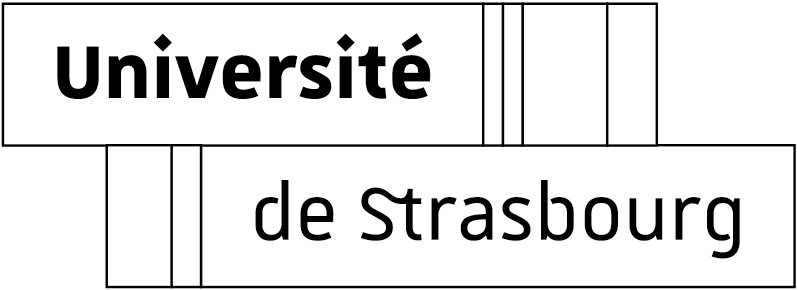
\includegraphics[scale=0.1]{../Images/Logo_Unistra.png}\phantom{AAAAAAAAAAAAAAAAAAAAAAAA}\footnotesize Academic year 2021-2022
\end{titlepage}

\bibliographystyle{ieeetr}
\tableofcontents

\chapter{Project's Presentation}
This project is part of the Master in Scientific Computing and Mathematics for Information.
One of the objectives of this master is to provide its students with advanced skills in data analysis.
This work is an excellent opportunity to put into practice what has been learned throughout the master's degree.

\section{Abstract}
The variety of human morphologies is an important issue for the textile-apparel industry.
Indeed, sizing systems currently used by companies have to be continuously updated or adapted to the population target.\bib{FFIT1, CIE}

For this reason, the Textile-Apparel-Industry requires a very accurate sizing system to minimize their costs and satisfy their customers.
However, the specific constraints of human morphotologies complicate the sizing system definition procedure and distributors prefer to use standard sizing system rather than an intelligent system suitable to their customers.

Until now, the morphotypes of a population are extracted from measurement charts.
However, new technologies such as 3D body scanning open new opportunities to enhance the morphotype generation from a sample of population especially with the 3D data of bodies.

The aim of this research is to define an exhaustive methodology to obtain a clustering of human morphology shapes representative of a population and to extract the most significant morphotype of each class.
Clustering methods are implemented and the performances are evaluated using real data.

These algorithms are validated in the context of the development of a module that takes an individual's measurements as input and proposes his morphotype.

\section{Main steps}
\begin{enumerate}[nolistsep]
	\item State of the art of different techniques and methods.
	\item Testing two promising algorithms.
	\item Validation of these algorithms.
\end{enumerate}

\subsection*{Related issues}
\begin{itemize}
	\setlength\itemsep{-0.25em}
	\item Same groups for men and women?
	\item Standardisation?
\end{itemize}

\section{Tools to be used}
\begin{itemize}
	\setlength\itemsep{-0.25em}
	\item Statistics
	\item Machine learning (supervised and unsupervised)
	\item Clustering
	\item Topological Data Analysis
	\item Programming in Python
\end{itemize}

\section{DiTeX: Data-Innovation for the Textile Industry}
DiTeX is a joint research and development laboratory between the University of Technology of Troyes and the French Institute of Textiles and Clothing.

This laboratory develops statistical modelling and machine learning to analyse data from clothing and to respond to problems dealing, in particular, with the measurements of the human body: What is the effect of ageing? What are the types of morphologies?

\subsection{University of Technology of Troyes}
Founded in 1994, the \href{https://www.utt.fr/}{University of Technology of Troyes} (Université de Technologie de Troyes\bib{UTT}; UTT) is a French university, in the Academy of Reims.

The UTT is part of the network of the three universities of technology, found by the University of Technology of Compiègne.
Inspired by the American University of Pennsylvania in Philadelphia, these three universities (UTC, UTBM and UTT) are a French mixture between the universities of this country and its schools of engineers (Grandes Ecoles).

\subsection{French Institute of Textiles and Clothing}
The \href{https://www.la-federation.com/fr/nos-actions-de-lobby/partenaires/institut-francais-du-textile-habillement-ifth-1343.html}{French Institute of Textiles and Clothing} (Institut Français du Textile et de l'Habillement\bib{IFTH}; IFTH) is an industrial technical centre created by decree on 14 April 2001.
Its mission is to promote and assist progress in the textile and clothing sectors.
\newpage

\rmfamily
\chapter{State of the Art}
\section{Female body shapes}
Body shapes are often categorised in the fashion industry into one of five elementary geometric shapes, though there are very wide ranges of actual sizes within each shape:

\begin{itemize}
	\setlength\itemsep{-0.25em}
	\item \textbf{Triangle, "A" Frame, Pear, Spoon or Christmas Tree}\\
	      The hips are wider than the bust.
	      The distribution of fat varies, with fat tending to deposit first in the buttocks, hips, and thighs.
	      As body fat percentage increases, an increasing proportion of body fat is distributed around the waist and upper abdomen.
	\item \textbf{Inverted Triangle, Cone or "V" Frame}\\
	      The shoulders are broader than the hips.
	      The legs and thighs tend to be slim, while the chest looks larger compared with the rest of the body.
	      Fat is mainly distributed in the chest and face.
	\item \textbf{Oval, Circle/Rounded, Apple, Diamond or "O" Frame}\\
	      Top and bottom are narrow.
	      Chest and belly are where weight is found.
	      Legs are skinny.
	\item \textbf{Rectangular, Ruler or "H" Frame}\\
	      The waist is less than 23cm smaller than the hips and bust.
	      Body fat is distributed predominantly in the abdomen, buttocks, chest, and face.
	      This overall fat distribution creates the typical ruler (straight) shape.
	\item \textbf{Hourglass, Figure 8 or "X" Frame}\\
	      The hips and bust are almost of equal size, and the waist is narrower than both.
	      Body fat distribution tends to be around both the upper body and lower body.
	      This body type enlarges the arms, chest, hips, and rear before other parts, such as the waist and upper abdomen.
\end{itemize}

\section{Analytical methods in somatology}
\subsection{Early figure typing}
Based on visual observation, Hippocrates\bib{Croney} recorded two distinct shapes of the human body in the 3rd century BC: thin/tall and short/thick.
Since this apparent beginning, methods of describing and classifying the various attributes of the human body have developed.

\subsection{Somatotype}
The somatotype, from the Greek soma, is an attempt to relate personality to the shape of the human body and its physical makeup once adolescent growth is complete.

William Sheldon\bib{Sheldon}, in the 1940s, initiated this line of research which is now widely considered simplistic.
He defined the somatotype as the arrangement of three poles that apply to both sexes:
\begin{itemize}
	\setlength\itemsep{-0.25em}
	\item \textbf{endomorph}: large, heavy and chubby
	\item \textbf{mesomorph}: large, muscular, solid
	\item \textbf{ectomorph}: elongated, delicate, with reduced musculature
\end{itemize}
We can therefore theoretically classify all human beings according to these three somatotypes.
Diversity means that most will be a mixture of these three somatotypes, which define the extreme specificities.
It is therefore rare that a person, regardless of gender, has only the characteristics of one pole.

Sheldon's technique involved analyzing photographic images of male subjects, taken from the front, side and back, and visually synthesizing them into 3D mental representations of body shape.

Sheldon’s work is an example of early visual body type classification combining photography with Cartesian grid structure but is now considered by researchers to be a collection of stereotypes rather than an empirical observation.\bib{Mull}

\subsection{Women's measurements for garments and pattern construction}
In 1941, the O’Brien and Shelton study of women’s measurements\bib{ROB} was one of the first to systematically collect linear body measurement data to be used for sizing apparel.
No scientific study of body measurements used in the construction of women's clothing had ever been reported.\bib{ROB2}

This study included not only the measuring of 14.698 women, but also a detailed statistical analysis of the results.
Special attention was given to discovering key measurements of the body; that is, a few important measurements from which all the others can best be predicted.

The analysis showed that girth measurements of the body have little relation to vertical (height) measurements.
\begin{table}[H]
	\begin{center}
		\caption{\centering\footnotesize\itshape Principal measurements for 5 "regular" sizes based on stature of 64 inches for girls (G) 15, 16, and 17 years old and for women (W) 18 years old and over.}
		\textsf{\scriptsize
			\begin{tabular}{|p{0.21\linewidth}||p{0.04\textwidth}|p{0.04\textwidth}|p{0.04\textwidth}|p{0.04\textwidth}|p{0.04\textwidth}|p{0.04\textwidth}|p{0.04\textwidth}|p{0.04\textwidth}|p{0.04\textwidth}|p{0.04\textwidth}|}
				\hline
				\multirow{3}{*}{\textbf{Measurement} \textit{(inches)}} & \multicolumn{10}{c|}{Value for stature 64 inches and weight}                                                                                                                                                                                                                                                 \\\cline{2-11}
				                                                        & \multicolumn{2}{c|}{\itshape 100 pounds}                     & \multicolumn{2}{c|}{\itshape 110 pounds} & \multicolumn{2}{c|}{\itshape 120 pounds} & \multicolumn{2}{c|}{\itshape 130 pounds} & \multicolumn{2}{c|}{\itshape 140 pounds}                                                                     \\\cline{2-11}
				                                                        & \centering G                                                 & \centering W                             & \centering G                             & \centering W                             & \centering G                             & \centering W & \centering G & \centering W & \centering G & W     \\
				\hline
				\textbf{Vertical}                                       &                                                              &                                          &                                          &                                          &                                          &              &              &              &              &       \\
				\phantom{1}Cervival height                              & 54.70                                                        & 54.82                                    & 54.75                                    & 54.89                                    & 54.80                                    & 54.96        & 54.84        & 55.03        & 54.89        & 55.10 \\
				\phantom{1}Hip height                                   & 32.82                                                        & 32.28                                    & 32.79                                    & 32.23                                    & 32.76                                    & 32.18        & 32.72        & 32.13        & 32.69        & 32.08 \\
				\phantom{1}Tibiale height                               & 17.65                                                        & 17.55                                    & 17.66                                    & 17.53                                    & 17.68                                    & 17.51        & 17.69        & 17.49        & 17.71        & 17.47 \\
				\phantom{1}Total posterior arm length                   & 23.23                                                        & 23.05                                    & 23.30                                    & 23.12                                    & 23.3fi                                   & 23.19        & 23.43        & 23.26        & 23.49        & 23.33 \\
				\phantom{1}Vertical trunk girth                         & 54.75                                                        & 56.60                                    & 55.68                                    & 57.69                                    & 56.62                                    & 58.78        & 57.55        & 59.87        & 58.48        & 60.96 \\
				\textbf{Horizontal}                                     &                                                              &                                          &                                          &                                          &                                          &              &              &              &              &       \\
				\phantom{1}Chest girth at armscye                       & 30.59                                                        & 30.84                                    & 31.70                                    & 31.97                                    & 32.81                                    & 33.10        & 33.91        & 34.23        & 35.02        & 35.36 \\
				\phantom{1}Bust girth                                   & 31.11                                                        & 30.68                                    & 32.31                                    & 32.08                                    & 33.51                                    & 33.48        & 34.71        & 34.88        & 35.91        & 36.28 \\
				\phantom{1}Waist girth                                  & 23.51                                                        & 23.39                                    & 24.60                                    & 24.99                                    & 25.69                                    & 26.59        & 26.78        & 28.19        & 27.87        & 29.79 \\
				\phantom{1}Hip girth                                    & 33.80                                                        & 34.71                                    & 35.16                                    & 35.91                                    & 36.53                                    & 37.11        & 37.89        & 38.31        & 39.25        & 39.51 \\
				\phantom{1}Max.
				thigh girth                                             & 18.90                                                        & 19.61                                    & 20.04                                    & 20.38                                    & 21.17                                    & 21.15        & 22.31        & 21.92        & 23.44        & 22.69 \\
				\phantom{1}Neck-base girth                              & 14.04                                                        & 14.48                                    & 14.26                                    & 14.72                                    & 14.49                                    & 14.96        & 14.71        & 15.20        & 14.92        & 15.44 \\
				\hline
			\end{tabular}}
	\end{center}
\end{table}

\subsection{Douty’s body build scales}
In 1968, Douty and Brannon used face forward and side silhouette photographs to study female and male body build and posture.
Their studies\bib{Douty} advanced somatographic measurement methods and focused on the constructs of body build and posture by visually classifying body types.

Douty’s body build scales were derived through visual analysis of photographs projected onto a Cartesian grid structure for reference.
\begin{figure}[H]
	\begin{minipage}{0.75\textwidth}
		\centering
		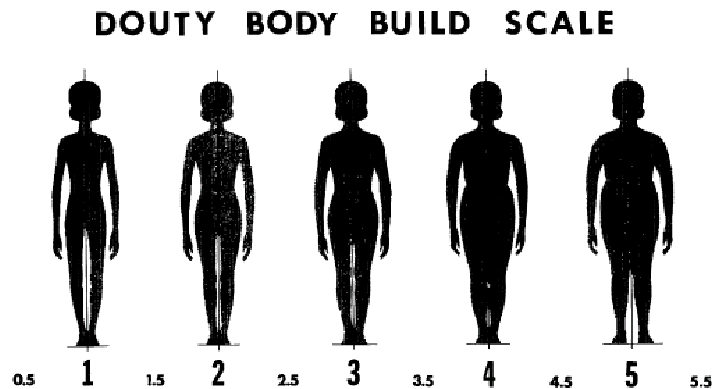
\includegraphics[width=.7\linewidth]{../Images/douty}
	\end{minipage}\hfill
	\begin{minipage}{0.25\textwidth}
		\begin{enumerate}[nolistsep]
			\item Thin
			\item Slender
			\item Average
			\item Stocky
			\item Heavy
		\end{enumerate}
	\end{minipage}
\end{figure}

\subsection{Dressmaking Focused Size and Shape Analysis}
\subsubsection{The Minott method}
In 1978, Minott categorized female human body shapes in components to aid in patternmaking for apparel\bib{Minott}.
In the development her method of fitting apparel patterns, she observed shoulder and hip size considering the relationship with other body parts.

Posture was also taken into account in order to adjust measurement data for more accurate patterns.

\subsubsection{August dress thin system}
In 1981, August assessed female body shape in relation to dressmaking\bib{Bonnie}.
She developed four categories of body type designated as A, X, V, and H.
These were observed from a front view of the subject.

Side views were qualitatively evaluated, as well, and utilized lower case designations like b, d, i, and r to indicate categories.

The August method of categorizing body shapes was based on landmark identification and recognition by component (\href{https://en.wikipedia.org/wiki/Recognition-by-components_theory}{RBC}).

\subsubsection{Patternmaking for fashion designers}
In 1987, Armstrong described four female body shapes based on the shoulder/hip relationship\bib{Armstrong}.
The categories she used included hourglass, straight line, wide shoulders, and narrow shoulders.

While these categories could be advantageous to patternmaking, they are limited to that application.

\subsection{Female Figure Identification Technique for apparel measurements}
\subsubsection{Original study}

In 2004, Simmons, Istook, and Devarajan developed a shape sorting software\bib{FFIT1,FFIT2}, called the Female Figure Identification Technique (FFIT) for apparel, to classify 3D body scans and identify body shapes.

The measurements were 1-dimensional measures taken from 3-dimensional body scans.

Having proven that basic systems were not adequate, they determined shape classification elements from the literature as a starting point, and then evaluated the relative visual and descriptive information to help determine a mathematical logic that could successfully identify shapes.
Using mathematical criteria and the tacit knowledge of garment design and fitting experts, a set of shapes was defined with mathematical descriptors.
\begin{enumerate}[nolistsep]
	\item Hourglass: proportional bust and hip measurements, with a defined waistline.
	\item Bottom Hourglass: larger hip than bust, with a defined waistline.
	\item Top Hourglass: larger bust than hip, with a defined waistline.
	\item Spoon: a significant difference between hip and bust, a bust-to-waist ratio smaller than Hourglass, and a significant high hip-to-waist ratio, indicating a “shelf” where the waist drops off sharply with similar hip and high hip measurements.
	\item Triangle: a larger hip than bust without a defined waist.
	\item Inverted Triangle: a larger bust than hip without a defined waist.
	\item Rectangle: similar bust and hip measurements, without a defined waistline.
	\item Diamond: a very large midsection with the average of stomach, waist, and abdomen larger than bust.
	\item Oval: a large midsection with the average of stomach, waist, and abdomen smaller than bust.
\end{enumerate}
Bust, waist, and hip circumferences were used to determine which body shape the scan matched.
Stomach and abdomen circumferences were also used to determine diamond and oval shapes.
However, Simmons \textit{et al}. did not provide a detailed description of where these measurements were taken on the scan.

To validate the identified body shapes, Simmons \textit{et al}. used a random sample of 887 subjects, collected from three sources.
They performed a discriminant analysis, dividing the sample into a training data (256 subjects) to develop the discriminant analysis function and a test data (531 subjects) to validate the discriminant.
Overall, the percentage accuracy of the FFIT$^\text{\copyright}$ software was better than the discriminant function.

\subsubsection{Comparison of body shape between USA and Korean women}

In a 2007 study\bib{IJCST} by Lee, Istook, Nam, and Park, body shapes of women from the U.S.
were compared to those from Korea, using measurement data from SizeUSA and SizeKorea with the FFIT for Apparel system.
In order to determine the efficacy of sorting USA and Korean women, Lee \textit{et al}. used a mathematical analysis and visual inspection to develop formulas based on the descriptions of the original FFIT software categories.
The formulas used bust, hip, waist, and high hip measurements to match body measures into one the following shape categories: Hourglass, Bottom Hourglass, Top Hourglass, Spoon, Triangle, Inverted Triangle, or Rectangle.
While Simmons \textit{et al}. initially included nine formulas, Lee \textit{et al}. did not include Diamond or Oval in their formulas.
\begin{table}[H]
	\centering
	\caption{\centering\footnotesize\itshape Original Female Figure Identification Technique (FFIT) formulas (in millimetres)}
	\textsf{\scriptsize
		\begin{tabular}{|l|l|}
			\hline
			\textbf{BODY TYPE} & {\textbf{MEASUREMENT}}                                                                                                    \\
			\hline
			Hourglass          & If (bust-hip)$\leqslant 25$), then if (hip-bust)$< 91$, then if (bust-waist)$\geqslant 230$ or (hip-waist)$\geqslant 250$ \\
			\hline
			Bottom hourglass   & If (hip-bust)$\geqslant 91$ and (hip-bust)$< 250$, then if (bust-waist)$\geqslant 230$,then if (high hip/waist)$< 1.193$  \\
			\hline
			Top hourglass      & If (bust-hip)$> 25$ and (bust-hip)$< 250$, then if (bust-waist)$\geqslant 230$                                            \\
			\hline
			Spoon              & If (hip-bust)$> 51$, then if (hip-waist)$\geqslant 180$, then if (high hip/waist)$\geqslant 1.193$                        \\
			\hline
			Triangle           & If (hip-bust)$\geqslant 91$, then if (hip-waist)$< 230$                                                                   \\
			\hline
			Inverted Triangle  & If (bust-hip)$\geqslant 91$, then if (bust-waist)$< 230$                                                                  \\
			\hline
			Rectangle          & If (hip-bust)$< 91$ and (bust-hip)$< 91$, then if (bust-waist)$\geqslant 230$ and (hips-waist)$< 250$                     \\
			\hline
		\end{tabular}}
\end{table}
\subsubsection{Modification of the FFIT Formulas to Include Plus Size Bodies}

In 2020, Sokolowski and Bettencourt modified the FFIT mathematical formulas to be more inclusive of plus size women\bib{SSCB}.
The inspections indicated that some scans were inaccurately classified or not sorted into any shape category.
Since plus size women often have larger abdomens than bust or hips, the formulas were modified to include a check for that condition.
\begin{table}[H]
	\centering
	\caption{\centering\footnotesize\itshape Modified FFIT formulas (in millimetres), adapted from Lee \textit{et al}.}
	\textsf{\scriptsize
		\begin{tabular}{|l|l|}
			\hline
			\textbf{BODY TYPE} & {\textbf{MEASUREMENT}}                                                                                                          \\
			\hline
			Hourglass          & If (bust-hip)$\leqslant 25$, then if (hip-bust)$< 91$, then if (bust-waist)$\geqslant 230$ or (hip-waist)$\geqslant 250$        \\
			\hline
			Bottom Hourglass   & If (hip-bust)$\geqslant 91$ and (hip-bust)$< 250$, then if (hip-waist)$\geqslant 230$, then if (high hip/waist)$< 1.193$        \\
			\hline
			Top Hourglass      & If (bust-hip)$> 1$ and (bust-hip)$< 250$, then if (bust-waist)$\geqslant 230$                                                   \\
			\hline
			Spoon              & If (hip-bust)$> 51$, then if (hip-waist)$\geqslant 178$, then if (high hip/waist)$\geqslant 1.193$                              \\
			\hline
			Triangle           & If (hip-bust)$\geqslant 91$, then if $0 \leqslant$(hip-waist)$< 230$, or if (bust-waist)$< 0$, then if (hip-waist)$\geqslant 0$ \\
			\hline
			Inverted Triangle  & If (bust-hip)$\geqslant 91$, then if (bust-waist)$< 9$, then if (hip-waist)$\geqslant 0$                                        \\
			\hline
			Rectangle          & If (hip-bust)$< 91$, and (bust-hip)$< 91$, then if $0 \leqslant$(bust-waist)$< 230$ and $0 \leqslant$(hip-waist)$< 250$         \\
			\hline
			Diamond            & If (hip-waist)$< 0$, and (bust-waist)$< 0$                                                                                      \\
			\hline
			Oval               & If (hip-waist)$< 0$, and (bust-waist)$\geqslant 0$                                                                              \\
			\hline
		\end{tabular}}
\end{table}

\subsection{Body Shape Assessment Scale}
In 2006, Connell, Ulrich, Brannon, Alexander, and Presley used experts' knowledge to develop a set of scales to assess female body shapes as visualized in body scans\bib{BSAS}, resulting in an instrument that could be applied through software to the analysis of body scan data.

Using 42 body scans representing women aged 20-55 years of age, through a series of steps, researchers developed nine scales for body shape assessment from front and side views.

Three (Body Build, Body Shape, and Posture) were for whole body analysis, and six (Front Torso Shape, Hip Shape, Shoulder Slope, Bust Shape, Buttocks Shape, Back Curvature) were for analysis of component body parts.

For validation, five experts used the Body Shape Assessment Scale (BSAS\copyright) to rate 100 additional body scans.

These ratings were used to program software to classify female body scan data using the BSAS\copyright.

\subsection{Analysis and classification of three-dimensional trunk shape of women by using the human body shape model}
In 2009, Nakamura and Kurokawa used the 3D measurements of 560 Japanese women aged 19 to 63 years taken in laser metrology.
The subjects were scanned in a natural standing posture, wearing only panties.
The data obtained for each subject consisted of approximately 160,000 body surface points.
After the measurement, the body shape model was adjusted to each subject's measurements.
Then, 560 shape data sets were extracted from the models.

The trunk shape data consisted of $750$ (control points)$\times 3(x, y, z) = 2,250$ coordinates or variables.
Because this number is much larger than the number of subjects, Nakamura and Kurokawa reduced the shape data in two steps:
\begin{itemize}
	\setlength\itemsep{-0.25em}
	\item reduction of the analysis region
	\item elimination of control points
\end{itemize}
Having no reason to believe that there is a statistical difference in shape between the right and left trunks.
They chose to treat the right half of the trunk instead of the whole trunk without missing information on shape.
$414$ control points are needed to describe the shape of the right side of the trunk, excluding the neck.
Therefore, the authors had the shape data consisting of $(414 \times 3) = 1242$ coordinate variables.
To focus on the shape analysis, they redefined the coordinate origin for each subject.
\begin{figure}[H]
	\begin{minipage}{0.22\textwidth}
		The redefined origin corresponds to the $x$ and $y$ coordinates of the pubic foot point (a) and $z$ of the jugular fossa point (b).

		And all of the coordinates are normalised to the height difference between the cervicale (c) and the pubic foot point in order to eliminate the height factor.
	\end{minipage}\hfill
	\begin{minipage}{0.78\textwidth}
		\centering
		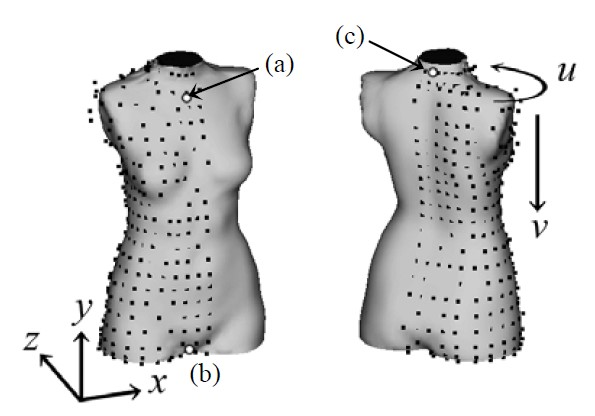
\includegraphics[width=0.75\linewidth]{../Images/Kuro1.jpg}
	\end{minipage}
\end{figure}

The second step of shape data reduction is based upon the correlation analysis between coordinates of the neighbouring control points in $(u, v)$ arrangement.
\begin{center}
	\noindent\fbox{
		\parbox{0.95\textwidth}{\itshape
			\begin{enumerate}[nolistsep]
				\item For each cell (target cell) on the map, we first look for coordinates that have a correlation coefficient greater than $0.80$ with the target cell.
				      And if the coordinates are within plus or minus two cells in the u and v directions of the target, we consider these coordinates to be representative of the target cell.
				\item Then we choose the control point that has the largest sum of the representable coordinates of $x, y$ and $z$ as the representative control point.
				\item The coordinates of the representative control point and their representable coordinates are removed from the map.
			\end{enumerate}
			These steps are repeated until the remaining coordinates have no representable coordinates.
		}}\end{center}

As a result, $111$ representative coordinates that can cover approximately $92\%$ of the original coordinates were chosen as the dataset for shape analysis.

Then, Nakamura and Kurokawa applied principal component analysis with varimax rotation to the variance-covariance matrix of the 111 representative coordinates of the 560 subjects to extract the shape factors of the female trunk.

The first principal component represents a trunk horizontality factor.

The second principal component is interpreted as a factor of breast height.

The third principal component corresponds to shoulder shape.

The fourth principal component can be considered to be a factor of longitudinal inclination of the trunk.

The fifth principal component may be a factor of breast size.

The sixth principal component is considered as a factor of fatness of the trunk.

The seventh or later components contain the form factors of the neck, shoulder, upper and lower abdomen, etc.
And they are not sufficient to characterize the whole trunk shape since these components involve only a small part of the body and their contribution rates are relatively low.
\begin{table}[H]
	\centering
	\caption{\centering\itshape Contribution rate of the main components}
	{\small
		\begin{tabular}{ccc}
			\hline
			Component & Contribution (\%) & Cumulative contribution (\%) \\
			\hline\hline
			1st       & 13.32             & 13.32                        \\
			2nd       & 11.36             & 24.67                        \\
			3rd       & 10.77             & 35.44                        \\
			4th       & 8.46              & 43.90                        \\
			5th       & 7.02              & 50.92                        \\
			6th       & 6.75              & 57.67                        \\
			7th       & 6.61              & 64.28                        \\
			8th       & 5.49              & 69.77                        \\
			\hline
		\end{tabular}}
\end{table}

Nakamura and Kurokawa then performed cluster analysis of the scores of the six principal components. We can easily derive classes by dividing a multidimensional principal component space\bib{Choi} where the 560 subjects are distributed according to their component scores.

However, this method unnecessarily produces many classes. The preferred number of classes is determined based on the dendrogram reflecting the relationship between the classes.

Nakamura and Kurokawa adopted \href{https://en.wikipedia.org/wiki/Ward%27s_method}{Ward's method}\bib{Ward} and used the squared Euclidean distance as the metric. The component scores are not normalized, as the variance of each component is of particular importance as a shape factor of the trunk.

As they wanted to have a relatively small number of classes, based on the dendrogram, they judged that ‘five’ is an appropriate number of classes. Therefore, they obtained five classes: C1, C2, C3, C4 and C5.
\begin{figure}[H]
	\centering
	\caption{\small\centering\itshape Dendrogram of cluster analysis and the level of the five classes}
	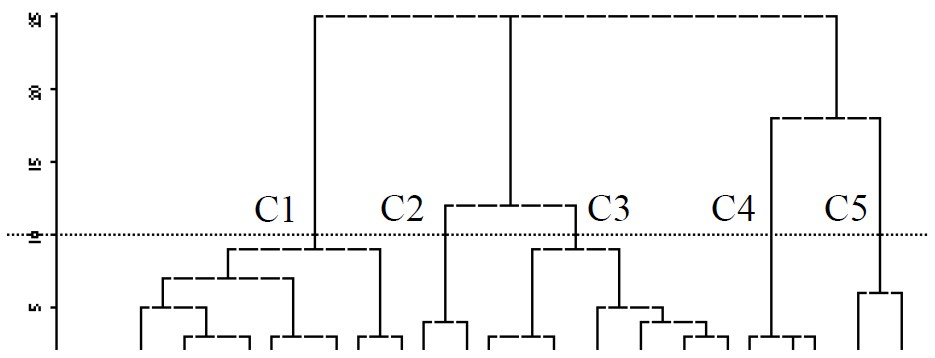
\includegraphics[width=0.9\linewidth]{../Images/Kuro2.jpg}
\end{figure}
\begin{figure}[H]
	\centering
	\caption{\small\centering\itshape Number of subjects in the classes}
	{\small
		\begin{tabular}{lccccc}
			\hline\hline
			\itshape Class  & C1  & C2 & C3  & C4 & C5 \\
			\hline
			No. of subjects & 180 & 45 & 195 & 63 & 77 \\
			\hline\hline
		\end{tabular}}
\end{figure}

\begin{figure}[H]
	\caption{Average figures in the classes C1 to C5}
	\centering
	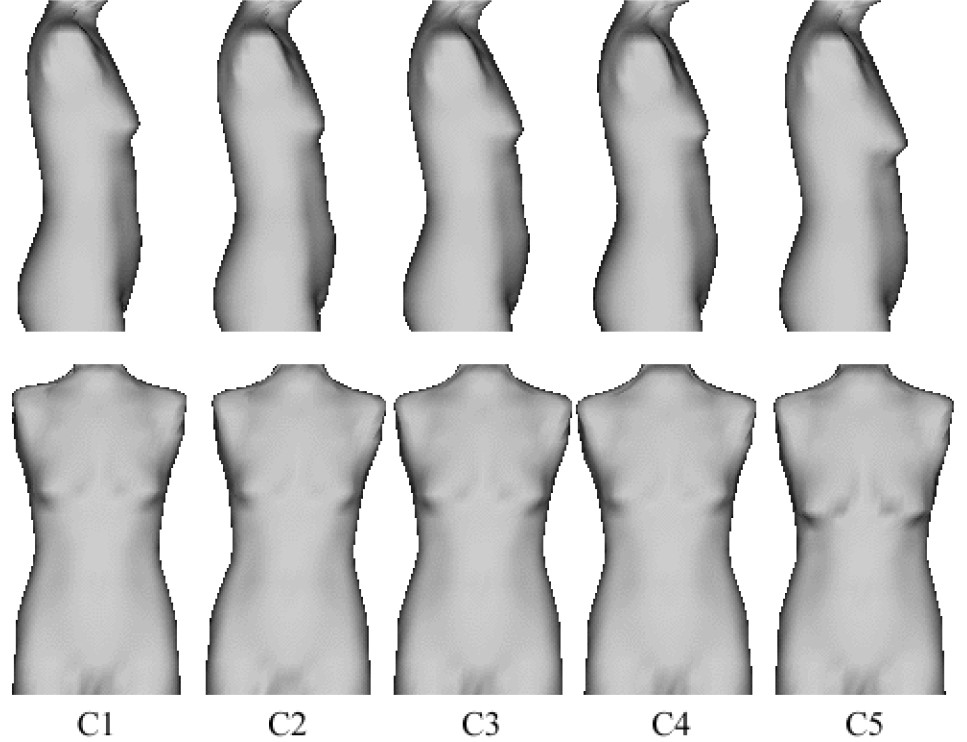
\includegraphics[width=0.75\linewidth]{../Images/Kuro3.jpg}
\end{figure}
C1 is a slim figure leaning forward and the angle of the shoulder slope is closer to horizontal. C2 is leaning to the left and has a relatively small chest at the highest level. C3 is a backward leaning posture and has about a third of the subjects, the largest number among the classes. C4 is leaning to the right and low shoulder and has the small chest. C5 has the appearance of a somewhat corpulent body and the chest position is lower than those of the other classes.

\subsection{Statistical human body form classification: Methodology development and application}
In 2012, Cottle\bib{phdthesis} developed a methodology to explore body shape analysis using 3D digital data generated by the body scanner. The exploratory research design consisted of pretesting, unsupervised clustering of male body scan data, and expert recognition of male body shape clusters.

The methodological framework is an adaptation of Costa and Cesar's framework for computational pattern analysis:
\begin{enumerate}[nolistsep]
	\item Form preprocessing
	\item Form transformations
	\item Form classification
\end{enumerate}

\subsubsection{Form preprocessing}
Acquisition, detection, noise filtering, and operations constitute form preprocessing.
Accurate data acquisition is critical to this stage of processing, and 3D body scanning has proven to be reliable in accomplishing this task\bib{FFIT1}.
The raw data from each subject's body scan can contain up to 1 million data points.

The data array is then processed by the body scanning software to filter out noise, resulting in a data file for each subject, consisting of an array of approximately $144\,000$ $(x, y, z)$ digital data points, which can be processed in the next step of the framework.

\subsubsection{Form transformations}
Normalization is achieved by the 3D body scanner software via the conversion of each subject's data file into an avatar mesh.
The avatar mesh contains over $32\,000$ data points.

Principal component analysis (PCA) techniques are then applied to reduce the number of data points while maintaining the descriptive integrity of the subject's body shape.
This results in a data file for each subject containing approximately $3\,000$ points.

The result of the form transformation is a file for each subject that has a common spatial point of origin, an equal number of data points, and a volume of data points that is manageable in further processing.

\subsubsection{Form classification}
Unsupervised classification or clustering is the method used in this study to develop a hierarchical clustering of subjects along the continuum of male body shapes.

Before proceeding, a pre-test of the method was conducted to explore the potential for success and to check for procedural problems.

\subsubsection{Pre-test}
The objective of this pre-test was to determine whether the body scan data could be acquired, transformed and classified.
The pre-test measured the ability of the cluster analysis algorithm to classify the data set into male and female body shape categories.

A sample of 10 male and 10 female body scans were selected based on every third qualifying data file contained in scan data collection of the Freshman 15 study\bib{Fresh}.
This sample was appropriate for the pre-test because the objective was to normalize the data and analyze it based on \textit{a priori} categories.

Two distinct categories of patterns emerged from the application of the unsupervised clustering methodology. A manual comparison of the contents of the two clusters revealed that the clusters were well separated by gender.

\subsubsection{Clustering of male body form}
The aim of this procedure was to apply the unsupervised hierarchical clustering methodology developed in the pre-test to a database of male body scan forms.

Male body scan data was used from the Men’s Mentoring Study\bib{MMS}.
This study focused exclusively on male subjects aged 18 or older and was determined to be demographically diverse enough to provide a good range of body form variability.
There were 117 body scan files out of 157 total files collected in the study that were convertible to the avatar mesh.

Applying the clustering technique established in the pretest to the $3\,104$ variables (height, weight, and 3D body scan data), seven distinct body form clusters emerged.
\begin{table}[H]
	\begin{center}
		\caption{\centering\itshape Average value of variables by cluster}
		{\small
			\begin{tabular}{cccccc}
				\hline
				Cluster & number & Age (years) & Weight (kg) & Height (cm) & BMI   \\
				\hline
				1       & 38     & 23.55       & 69.12       & 176.32      & 22.34 \\
				2       & 3      & 25.67       & 72.27       & 182.88      & 21.67 \\
				3       & 45     & 24.38       & 81.65       & 179.60      & 25.36 \\
				4       & 5      & 24.80       & 80.65       & 177.80      & 25.60 \\
				5       & 15     & 27.00       & 96.65       & 182.70      & 29.20 \\
				6       & 5      & 27.80       & 112.85      & 187.45      & 32.20 \\
				7       & 6      & 29.33       & 135.40      & 182.88      & 40.83 \\
				\hline
			\end{tabular}}
	\end{center}
\end{table}

\begin{figure}[H]
	\centering
	\caption{\small\centering\itshape Dendrogram depicting cluster analysis results. Cluster analysis using combined height, weight, and 3D body scan variables from the main study subject’s data.}
	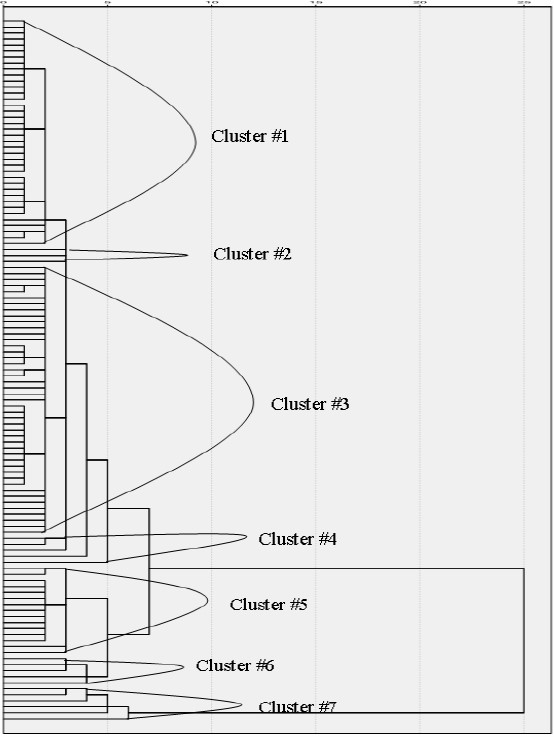
\includegraphics[width=0.65\linewidth]{../Images/Cottle.jpg}
\end{figure}
The seven distinct clusters are shown by the arched lines labeled by cluster number.
The arched lines are the result of the researcher’s subjective visual analysis of the cluster structure guidelines established in the pre-test.

The panel of experts was provided with the dendrogram shown in Figure 2.4 and detailed statistical descriptions of each group.
In addition, the panel received body scan images of  the first, middle and last subject in each group.
\begin{figure}[H]
	\centering
	\caption{\centering\itshape Expert visual analysis summary chart.}
	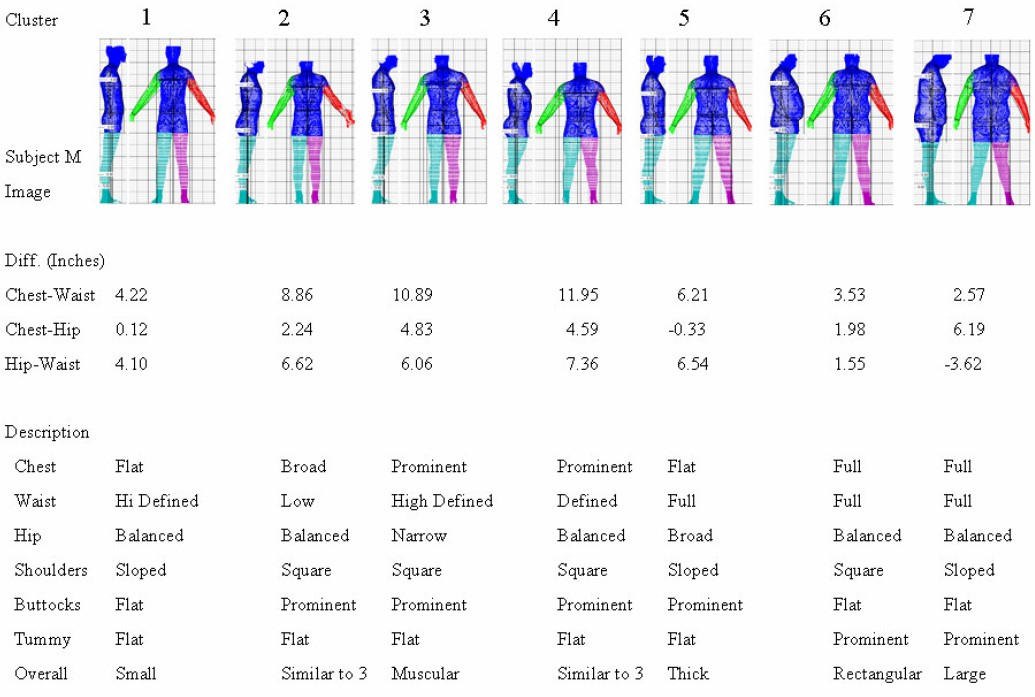
\includegraphics[width=0.95\linewidth]{../Images/Cottle2.jpg}
\end{figure}

The experts found that clusters 1 and 3 are the most visually consistent in shape.
These two clusters have the most similar and visually identifiable features.

The same is true, to a lesser extent, for cluster 5.

Clusters 2 and 4 seem to be the least cohesive.
Subjects in these clusters could easily be reclassified into adjacent clusters with which they share more definable common characteristics.

Clusters 6 and 7 are less well defined than clusters 1, 3 and 5.
This could be the result of the smaller number of subjects in the sample that fit these categories.
However, these clusters remain cohesive, with the exception of subject 7H.
Subject 7H seems to match the descriptors of cluster 5 better.

Therefore, most clusters have some degree of cohesion, but not complete cohesion.
The analysis shows that the sample can be grouped into five well-defined clusters.

\subsection{Body shape analyses of large persons in South Korea}
In 2013, Park and Park studied the body shapes of large people using anthropometric data from South Korea.\bib{ERGO}
For each gender, multivariate statistical analyses were conducted to identify key factors in body shape variability and to determine representative body types.

Two datasets, one male and one female, were prepared by identifying large individuals from the SizeKorea anthropometric database and collecting data on their body dimensions.
This study used the data preparation scheme proposed by Nam, Park and Jung, who analysed the body shapes of large men using data from the SizeKorea database.

To identify large individuals, only those aged 10-69 years were considered.
Three known indices of body size, Broca's Index ($\geqslant 20$), BMI ($\geqslant 25$) and waist-to-hip ratio (WHR $\geqslant 1.0$), were used to define large individuals.

A total of $1\,444$ males and $1\,327$ females were identified from the database.
The large individuals were segmented into four age groups: 10s, 20–30s, 40s–50s and 60s.
\begin{table}[H]
	\centering
	\caption{\centering\itshape Number individuals in each age group.}
	\begin{tabular}{lccccr}
		\hline\hline
		       & 10s   & 20s–30s & 40s–50s & 60s   & Total  \\
		\hline
		Male   & $366$ & $523$   & $390$   & $165$ & $1444$ \\
		Female & $271$ & $269$   & $441$   & $346$ & $1327$ \\
		\hline\hline
	\end{tabular}
\end{table}

Five ergonomics and industry domain experts participated in the selection of body dimensions. The criteria used were:
\begin{enumerate}[nolistsep]
	\item The dimensions should reflect changes in body shape due to the accumulation of body fat or changes in muscle mass
	\item The dimensions should be relevant to design applications in the clothing, furniture, automotive and consumer electronics sectors.
\end{enumerate}
A total of 33 and 36 body dimensions were selected for males and females, respectively.

For each gender, a factor analysis was conducted on the corresponding anthropometric data set.
The varimax orthogonal rotation method\bib{Hair} was used.
Body dimensions with a commonality of less than 0.5 were removed in the factor analysis process, and those with multiple loadings on all factors were either removed if interpretation of significance was difficult or placed with the factors that are conceptually closest.
Finally, each factor was standardised with a mean of 0 and a standard deviation of 1.

After the factor analyses, a cluster analysis was performed for each gender using the corresponding factor score data set.
Ward's method\bib{Ward}, which is a hierarchical clustering algorithm, was used.
The Euclidean distance between the factor score vectors of two individuals was used as a measure of dissimilarity.

Body shape classifications ranging from 3 to 6 body types were considered.
To select a particular classification within this range, the widely used cubic clustering criterion (CCC) and Hotelling's pseudo $T^2$ were employed\bib{Hair}.

For each gender, the selected body shape classification was evaluated to determine whether its body types (clusters) differ significantly from each other in terms of body shape characteristics.
To do this, for each factor, a one-way analysis of variance (ANOVA) with Student-Neuman-Keuls (SNK) post-hoc multiple comparison tests was performed to compare the mean scores of the body type factors.
Next, the shape characteristics of the body types were delineated on the basis of the mean factor scores of the groups.

\subsubsection{Male dataset results}
Five factors were identified, which collectively accounted for 81.53\% of the total variance.
\begin{table}[H]
	\centering
	\caption{\footnotesize\centering\itshape Cluster mean factor scores (centroid position) for each of the four male body types.}
	{\sffamily\scriptsize
		\begin{tabular}{lcccccc}
			\hline
			                     & \multicolumn{5}{c}{$Cluster$ $mean$ $factor$ $scores$}                                                                                                                \\
			\cline{2-6}
			                     & \textbf{Factor 1}:                                     & \textbf{Factor 2}: & \textbf{Factor 3}: & \textbf{Factor 4}: & \textbf{Factor 5}:     & Relative frequencies \\
			                     & $Waist$ $and$ $abdomen$                                & $Leg$              & $Upper$ $arm$      & $Torso$ $surface$  & $Biacromial$ $breadth$ & (\% total sample)    \\
			\hline
			\textbf{Body Type 1} & 0.7626                                                 & 1.0741             & 0.8794             & 0.4885             & 0.3838                 & 10.10\%              \\
			\textbf{Body Type 2} & 20.1820                                                & 0.7716             & 20.4770            & 20.3974            & 20.5495                & 26.68\%              \\
			\textbf{Body Type 3} & 0.0770                                                 & 20.4731            & 20.3619            & 1.0850             & 0.1782                 & 23.21\%              \\
			\textbf{Body Type 4} & 20.1318                                                & 20.5624            & 0.2877             & 20.4734            & 0.1592                 & 40.01\%              \\
			\hline
		\end{tabular}
	}
\end{table}

Among the classifications with three to six clusters generated by Ward's method, the one with four clusters (thus four body types) was selected:
\begin{enumerate}[label=\textbf{Type \arabic*:}, nolistsep]
	\item All of the five cluster mean factor scores of this body type were above zero.
	      Moreover, among the four types, it has the highest average cluster factor scores for factors 1, 2, 3 and 5 and the second highest for factor 4.
	      This body type is therefore described as the \textit{large everyway} type.
	\item Characterised by four below average (negative) cluster mean factor scores for factors 1, 3, 4 and 5 and one above average score for factor 2.
	      This body type is referred to as the \textit{small figure but above average legs} type.
	\item Labelled as a \textit{large torso area} type because its mean score on the grouping factor for the torso area factor (factor 4) is significantly greater than zero by more than one standard deviation.
	\item Of the four body types, this body type has the lowest average scores for factors 2 (legs) and 4 (torso).
	      It has been labelled as the \textit{small legs and small torso} type.
\end{enumerate}
\begin{figure}[H]
	\centering
	\caption{\footnotesize\centering\itshape Body scan images representing the four body types of large Korean males.}
	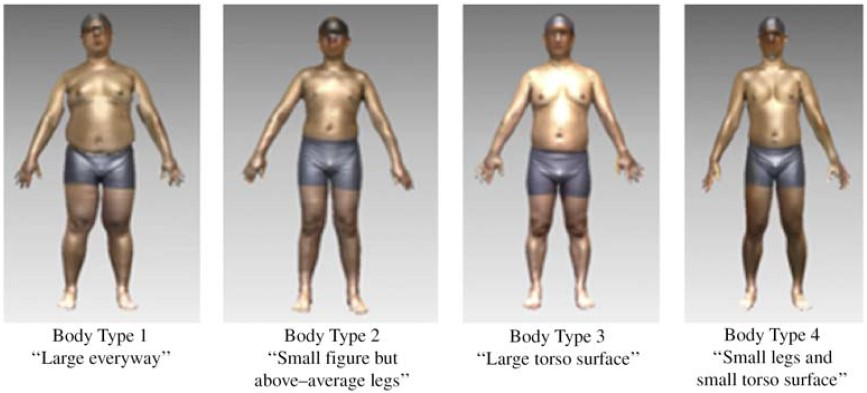
\includegraphics[width=.8\linewidth]{../Images/Park1}
\end{figure}

\subsubsection{Female dataset results}
Three factors were identified, which collectively accounted for 74.10\% of the total variance.
\begin{table}[H]
	\centering
	\caption{\footnotesize\centering\itshape Cluster mean factor scores (centroid position) for each of the four male body types.}
	{\sffamily\footnotesize
		\begin{tabular}{lcccc}
			\hline
			                     & \multicolumn{3}{c}{$Cluster$ $mean$ $factor$ $scores$}                                                                      \\
			\cline{2-4}
			                     & \textbf{Factor 1}:                                     & \textbf{Factor 2}: & \textbf{Factor 3}:     & Relative frequencies \\
			                     & $Torso$                                                & $Lower$ $body$     & $Biacromial$ $breadth$ & (\% total sample)    \\
			\hline
			\textbf{Body Type 1} & 1.1151                                                 & 0.1375             & 20.4820                & 25.93\%              \\
			\textbf{Body Type 2} & 0.1025                                                 & 20.3920            & 1.2377                 & 18.28\%              \\
			\textbf{Body Type 3} & 20.6921                                                & 0.5967             & 0.0922                 & 35.43\%              \\
			\textbf{Body Type 4} & 20.3548                                                & 20.9093            & 20.6830                & 20.37\%              \\
			\hline
		\end{tabular}
	}
\end{table}

Among the classifications with three to six clusters generated by Ward's method, the one with four clusters (thus four body types) was selected:
\begin{enumerate}[label=\textbf{Type \arabic*:}, nolistsep]
	\item Among the four body types, it has the highest average cluster factor score for factor 1.
	      It is second to last for factor 3.
	      It is labelled as the \textit{large torso and below-average shoulder width} type.
	\item Of the four body types, it has the highest average cluster factor score for factor 3 and the second lowest for factor 2.
	      It is labelled the \textit{wide shoulder and below-average lower body} type.
	\item Labelled as the \textit{small torso and large lower body} type because it has the lowest average cluster factor score for factor 1 and the highest for factor 2.
	\item All three cluster mean factor scores are negative for this body type.
	      Furthermore, it has the lowest average factor scores for factors 2 and 3 and the second lowest for factor 1.
	      It is labelled the \textit{small figure} type.
\end{enumerate}
\begin{figure}[H]
	\centering
	\caption{\footnotesize\centering\itshape Body scan images representing the four body types of large Korean females.}
	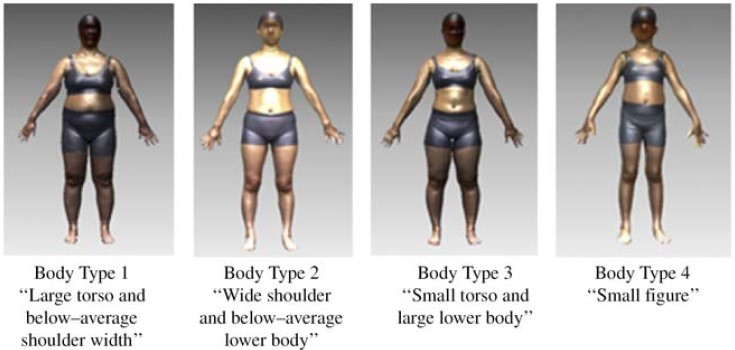
\includegraphics[width=.8\linewidth]{../Images/Park2}
\end{figure}

\chapter{Human body form classification}
For this study, we will use two clustering methods on two data sets, one female and one male.

In this chapter we present the results we have obtained. Due to time constraints, we did not have time to discuss the results.

\section{Clustering methods}
\subsection{K-Medoids (PAM)}
In statistics, a medoid is the most central representative of a class. The K-Medoid algorithm is a more robust partitioning algorithm with respect to outliers than the K-Means algorithm.

Like the K-Means, the K-Medoids algorithm minimises the mean square error which is the distance between the points of the class and the central point (or medoid).

The PAM\bib{PAM} algorithm is based on finding k medoids among the observations in the dataset.

After finding a set of k medoids, clusters are constructed by assigning each observation to the closest medoid.
If the sum of dissimilarities of all objects with their closest medoid can be reduced by swapping a selected object (medoid) with a non-selected object, then a swap is performed. This is continued until the sum of dissimilarities cannot be reduced any further.

The aim is to find k representative objects that minimise the sum of the dissimilarities of the observations with respect to their nearest representative object.

\subsection{Ward's method}
Ward's method\bib{Ward} is a hierarchical clustering algorithm.

Ward's minimum variance criterion minimises the total variance within clusters. In order to implement this method, at each step, the pair of clusters that results in a minimum increase in total variance within the cluster after merging must be found.

The Euclidean distance between the factor score vectors of two individuals was used as a measure of dissimilarity.

\subsection{Finding the optimal number of clusters}
For the same dataset, there are many possible partitionings\bib{KSel}.
It is therefore necessary to choose the most relevant number of clusters K to highlight the interesting patterns.
Unfortunately, there is no automatic procedure for this.

\subsubsection{Elbow method}
The "Elbow method" is an empirical method that consists of running the clustering algorithm with different K values, calculating the variance between the clusters, and then placing the different numbers of K clusters according to the variance on a graph. The result is an elbow-shaped visualisation, where the optimal number of clusters is the point representing the tip of the elbow.

\begin{figure}[H]
	\centering
	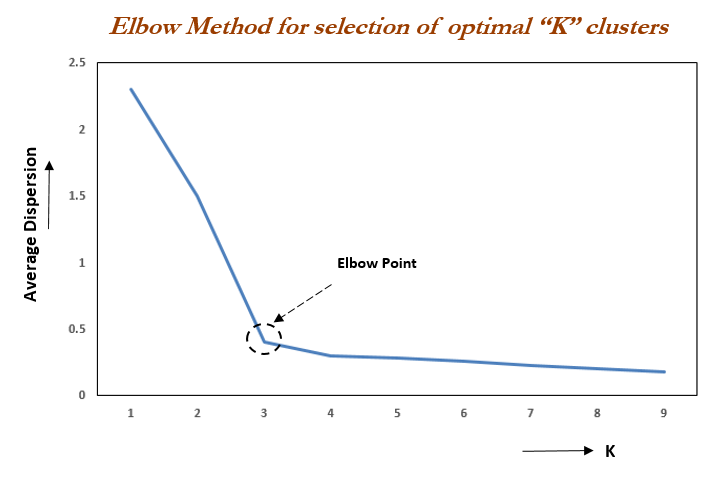
\includegraphics[width=0.9\textwidth]{../Images/Elbow_Method.png}\bib{Elbow}
\end{figure}

\subsubsection{Silhouette Coefficient}
The Silhouette Coefficient for a point $i$ is defined as follows:
$$
	S(i) = \frac{b(i)-a(i)}{\max\{a(i), b(i)\}}
$$
where $b(i)$ is the smallest average distance of point $i$ from all points in any other cluster and $a(i)$ is the average distance of $i$ from all other points in its cluster.

The silhouette coefficient of the data set is the average of the silhouette coefficient of the individual points. It tells us whether the individual points are correctly assigned to their clusters.

We can use the following rules of thumb when using the silhouette coefficient:
\begin{itemize}
	\item S(i) close to 0 means that the point is between two clusters.
	\item if it is closer to -1, it is better to assign it to other clusters.
	\item if S(i) is close to 1, then the point belongs to the "good" cluster.
\end{itemize}

\subsubsection{Calinski-Harabasz Index}
The Calinski-Harabasz index is based on the idea that clusters that are themselves very compact and well spaced from each other are good clusters.

The index is calculated by dividing the variance of the sums of the squares of the distances of individual objects from their cluster centre by the sum of the squares of the distance between the cluster centres.

It is defined as:
$$
	CH_k = \frac{BCSM}{k-1}\times\frac{n-k}{WCSM}
$$

where $k$ is the number of clusters, $n$ is the number of records in data, $BCSM$ (between cluster scatter matrix) calculates separation between clusters and $WCSM$ (within cluster scatter matrix) calculates compactness within clusters.

The higher the index value, the better the clustering model.

\subsubsection{Davies-Bouldin Index}
The Davies-Bouldin index is a measure of the quality of a partition of a data set in automatic classification.

It is the average of the maximum ratio between the distance of a point to the center of its group and the distance between two group centers.

It is defined as
$$
	DB = \frac1n\sum_{i=1}n\max_{j\neq i}\left(\frac{\sigma_i+\sigma_j}{d(c_i, c_j)}\right)
$$
where $n$ is the count of clusters and $\sigma_i$ is the average distance of all points in cluster $i$ from the cluster centre $c_i$.

The Davies-Bouldin index varies between 0 (best classification) and $\textstyle +\infty$ (worst classification).

For a cluster k, this index is all the lower as all clusters are homogeneous and all are well separated.

\subsubsection{Choice of the method}
The silhouette coefficient, the Calinski-Harabasz index and the Davies-Bouldin index account for both the separation and the compactness of clusters. Stastistically, it is almost certain that the clusters we obtain will not be separated.

Therefore, we will use the elbow method.

\section{Datasets}
Data from the Anthropometric Survey of U.S. Army Personnel\bib{ANSUR} (ANSUR II) were published internally in 2012.
They were made available to the public in 2017.
They include 93 measurements for over 6,000 US military adults (4,082 men and 1,986 women).
Despite the presence of reservists in the sample, it is not a approximation for the US civilian population.

For more information on this database, see: \url{https://www.openlab.psu.edu/ansur2/}

\subsection{Missing values}
First let's look if there are missing values:
\begin{figure}[H]
	\centering
	\caption{Data missing values}
	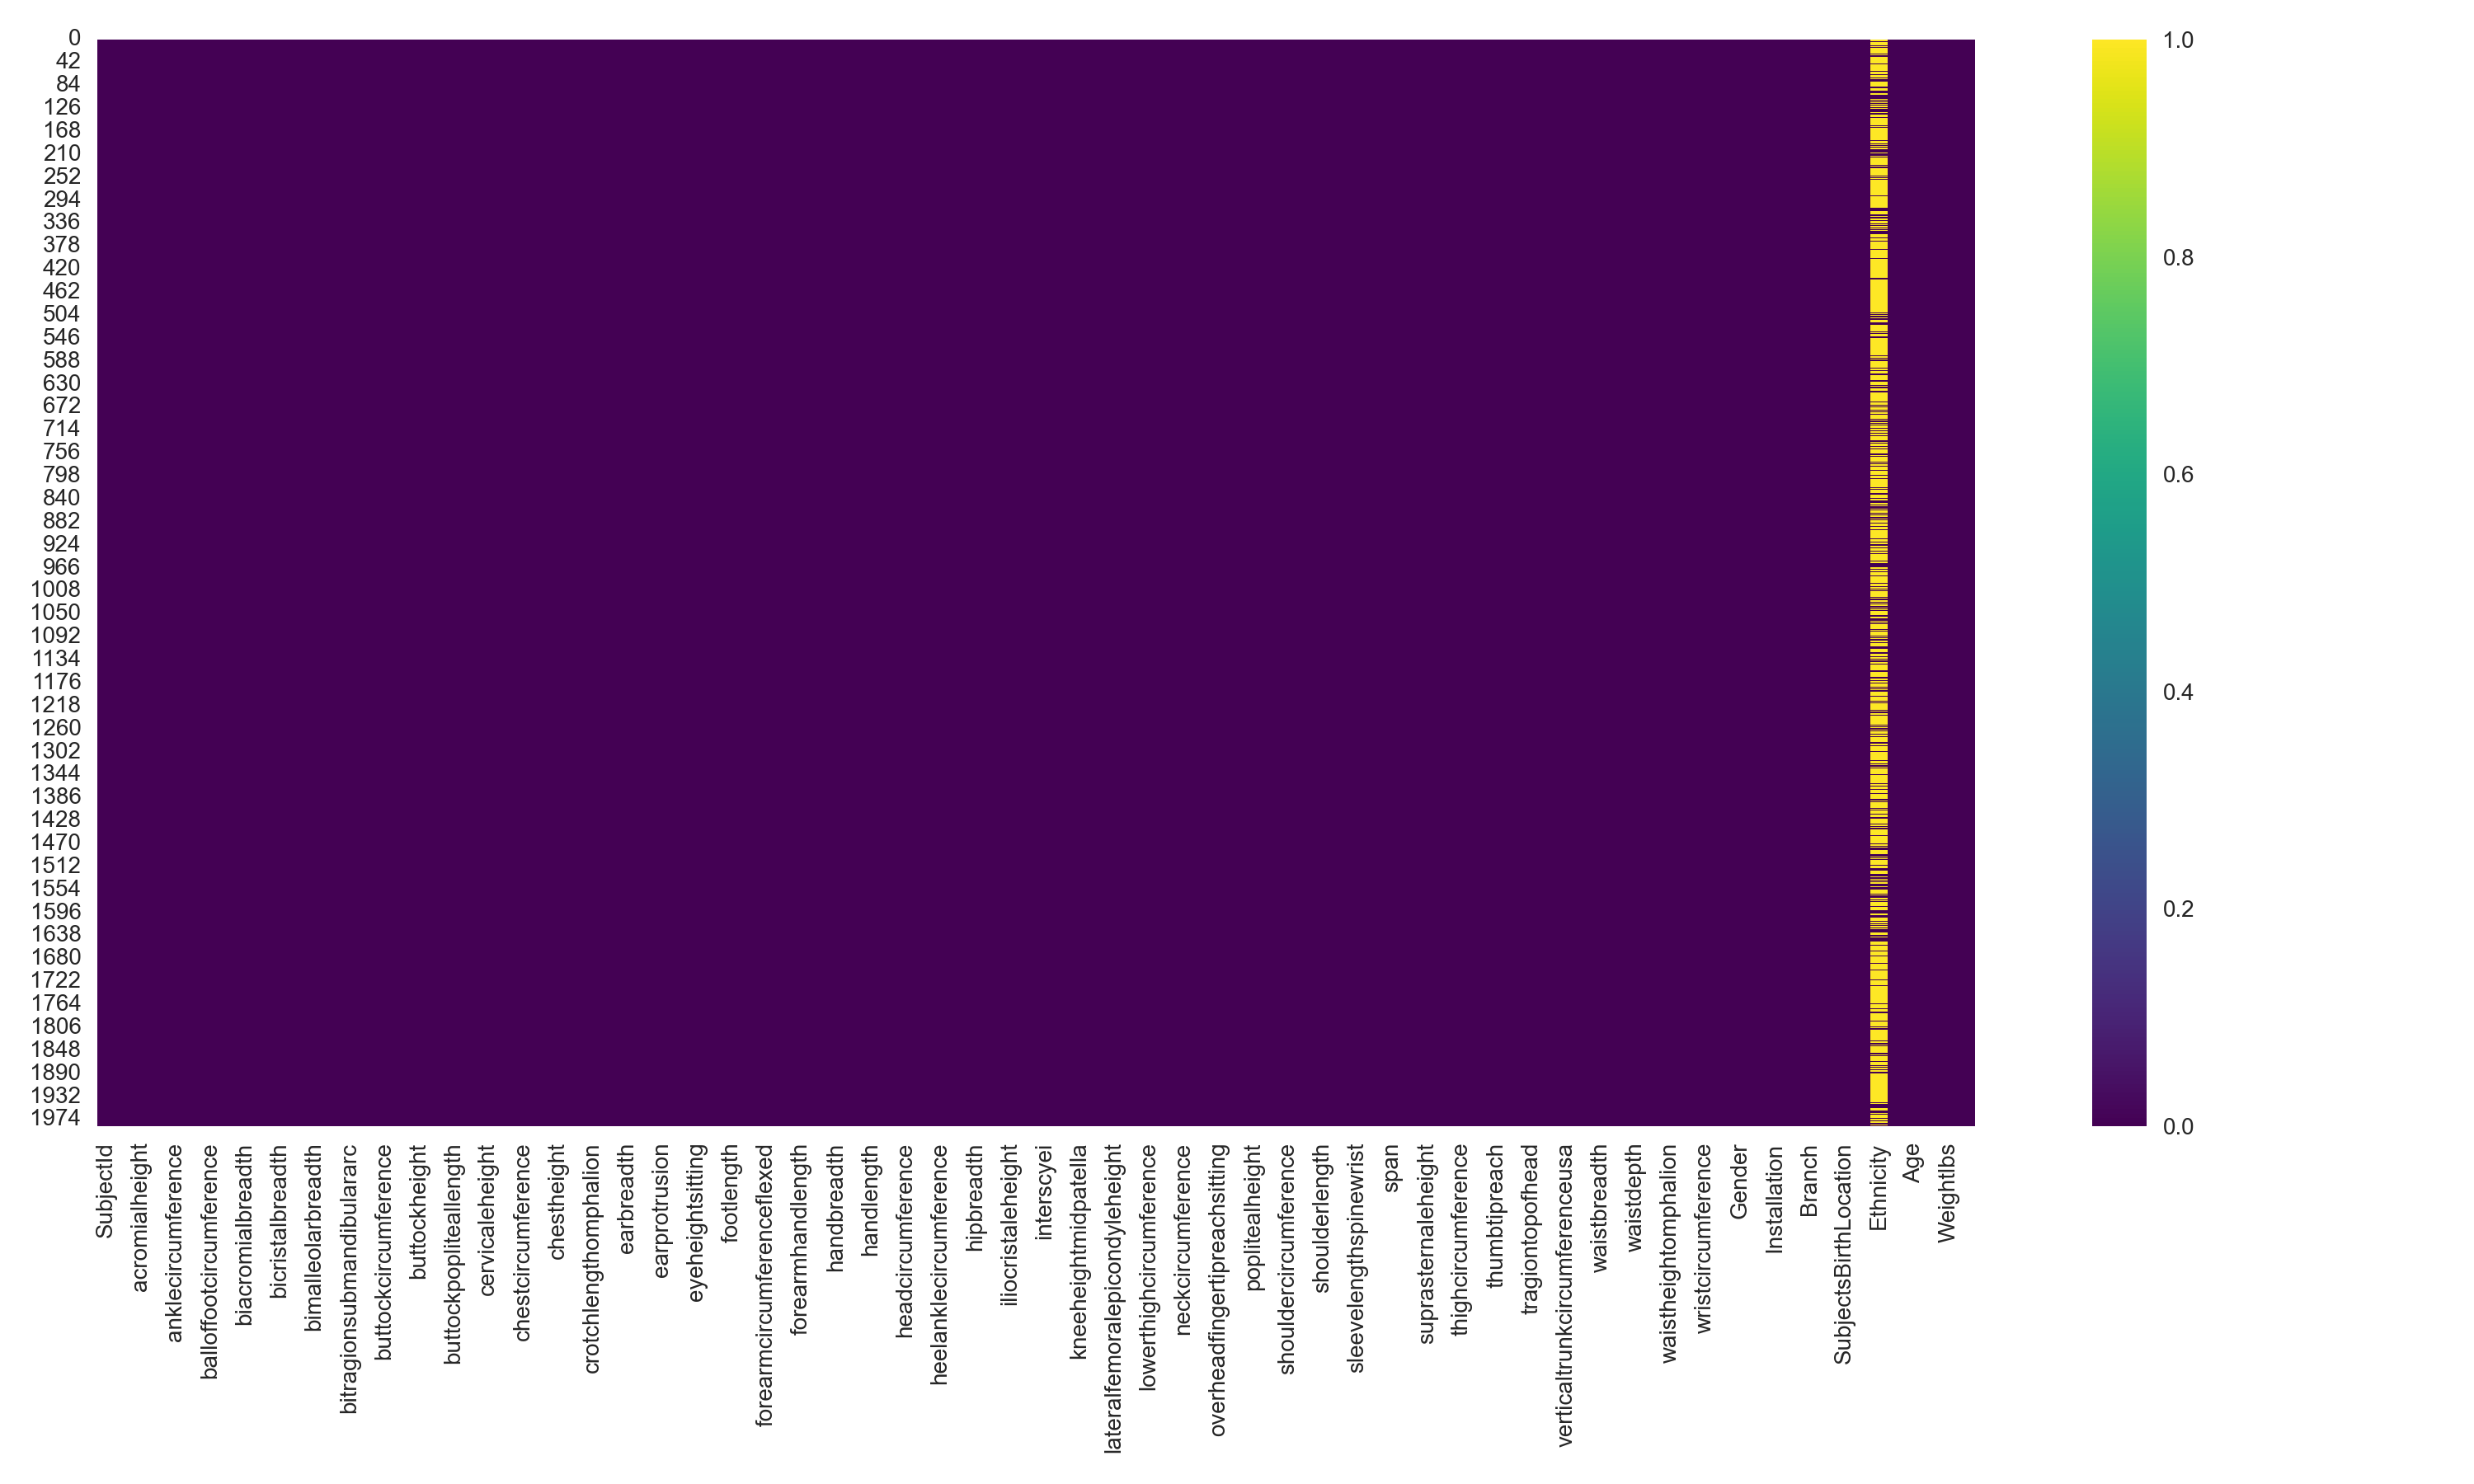
\includegraphics[width=\textwidth, height=0.4\textheight]{../Images/Missing_Values.png}
\end{figure}
The only missing values are those for ethnicity.

\subsection{Data sets preparation}
Some of the data are not relevant for our study, such as age, race, place of birth, race...

We decide to keep only 14 torso and thigh measurements: bicristal breadth, buttock circumference, buttock depth, chest breadth, chest circumference, chest depth, hip breadth, lower thigh circumference, shoulder circumference, thigh circumference, vertical trunk circumference, waist breadth, waist circumference and waist depth.

All these measurements are in centimetres and have integer values.

If two variables are not in the same scale, one might have more weight in the calculation of the Euclidean distance than the other. This is why we centre-reduce the data. Indeed, "centering-reduction" allows to obtain data that are independent of their unit.

\section{Female data set}
\vspace{-8mm}
\begin{table}[H]
	\caption{Female data set}
	\centering
	\begin{tabular}{|cccc|c|}
		\hline
		Age   & Height (cm) & Weight (kg) & BMI   & \textit{Count} \\
		\hline
		28.94 & 164.09      & 66.91       & 24.82 & \textit{1986}  \\
		\hline
	\end{tabular}
\end{table}

\subsection{Correlation matrix}
We calculate the correlation matrix of the measurements.
\begin{figure}[H]
	\centering
	\caption{Correlation matrix for the female data set}
	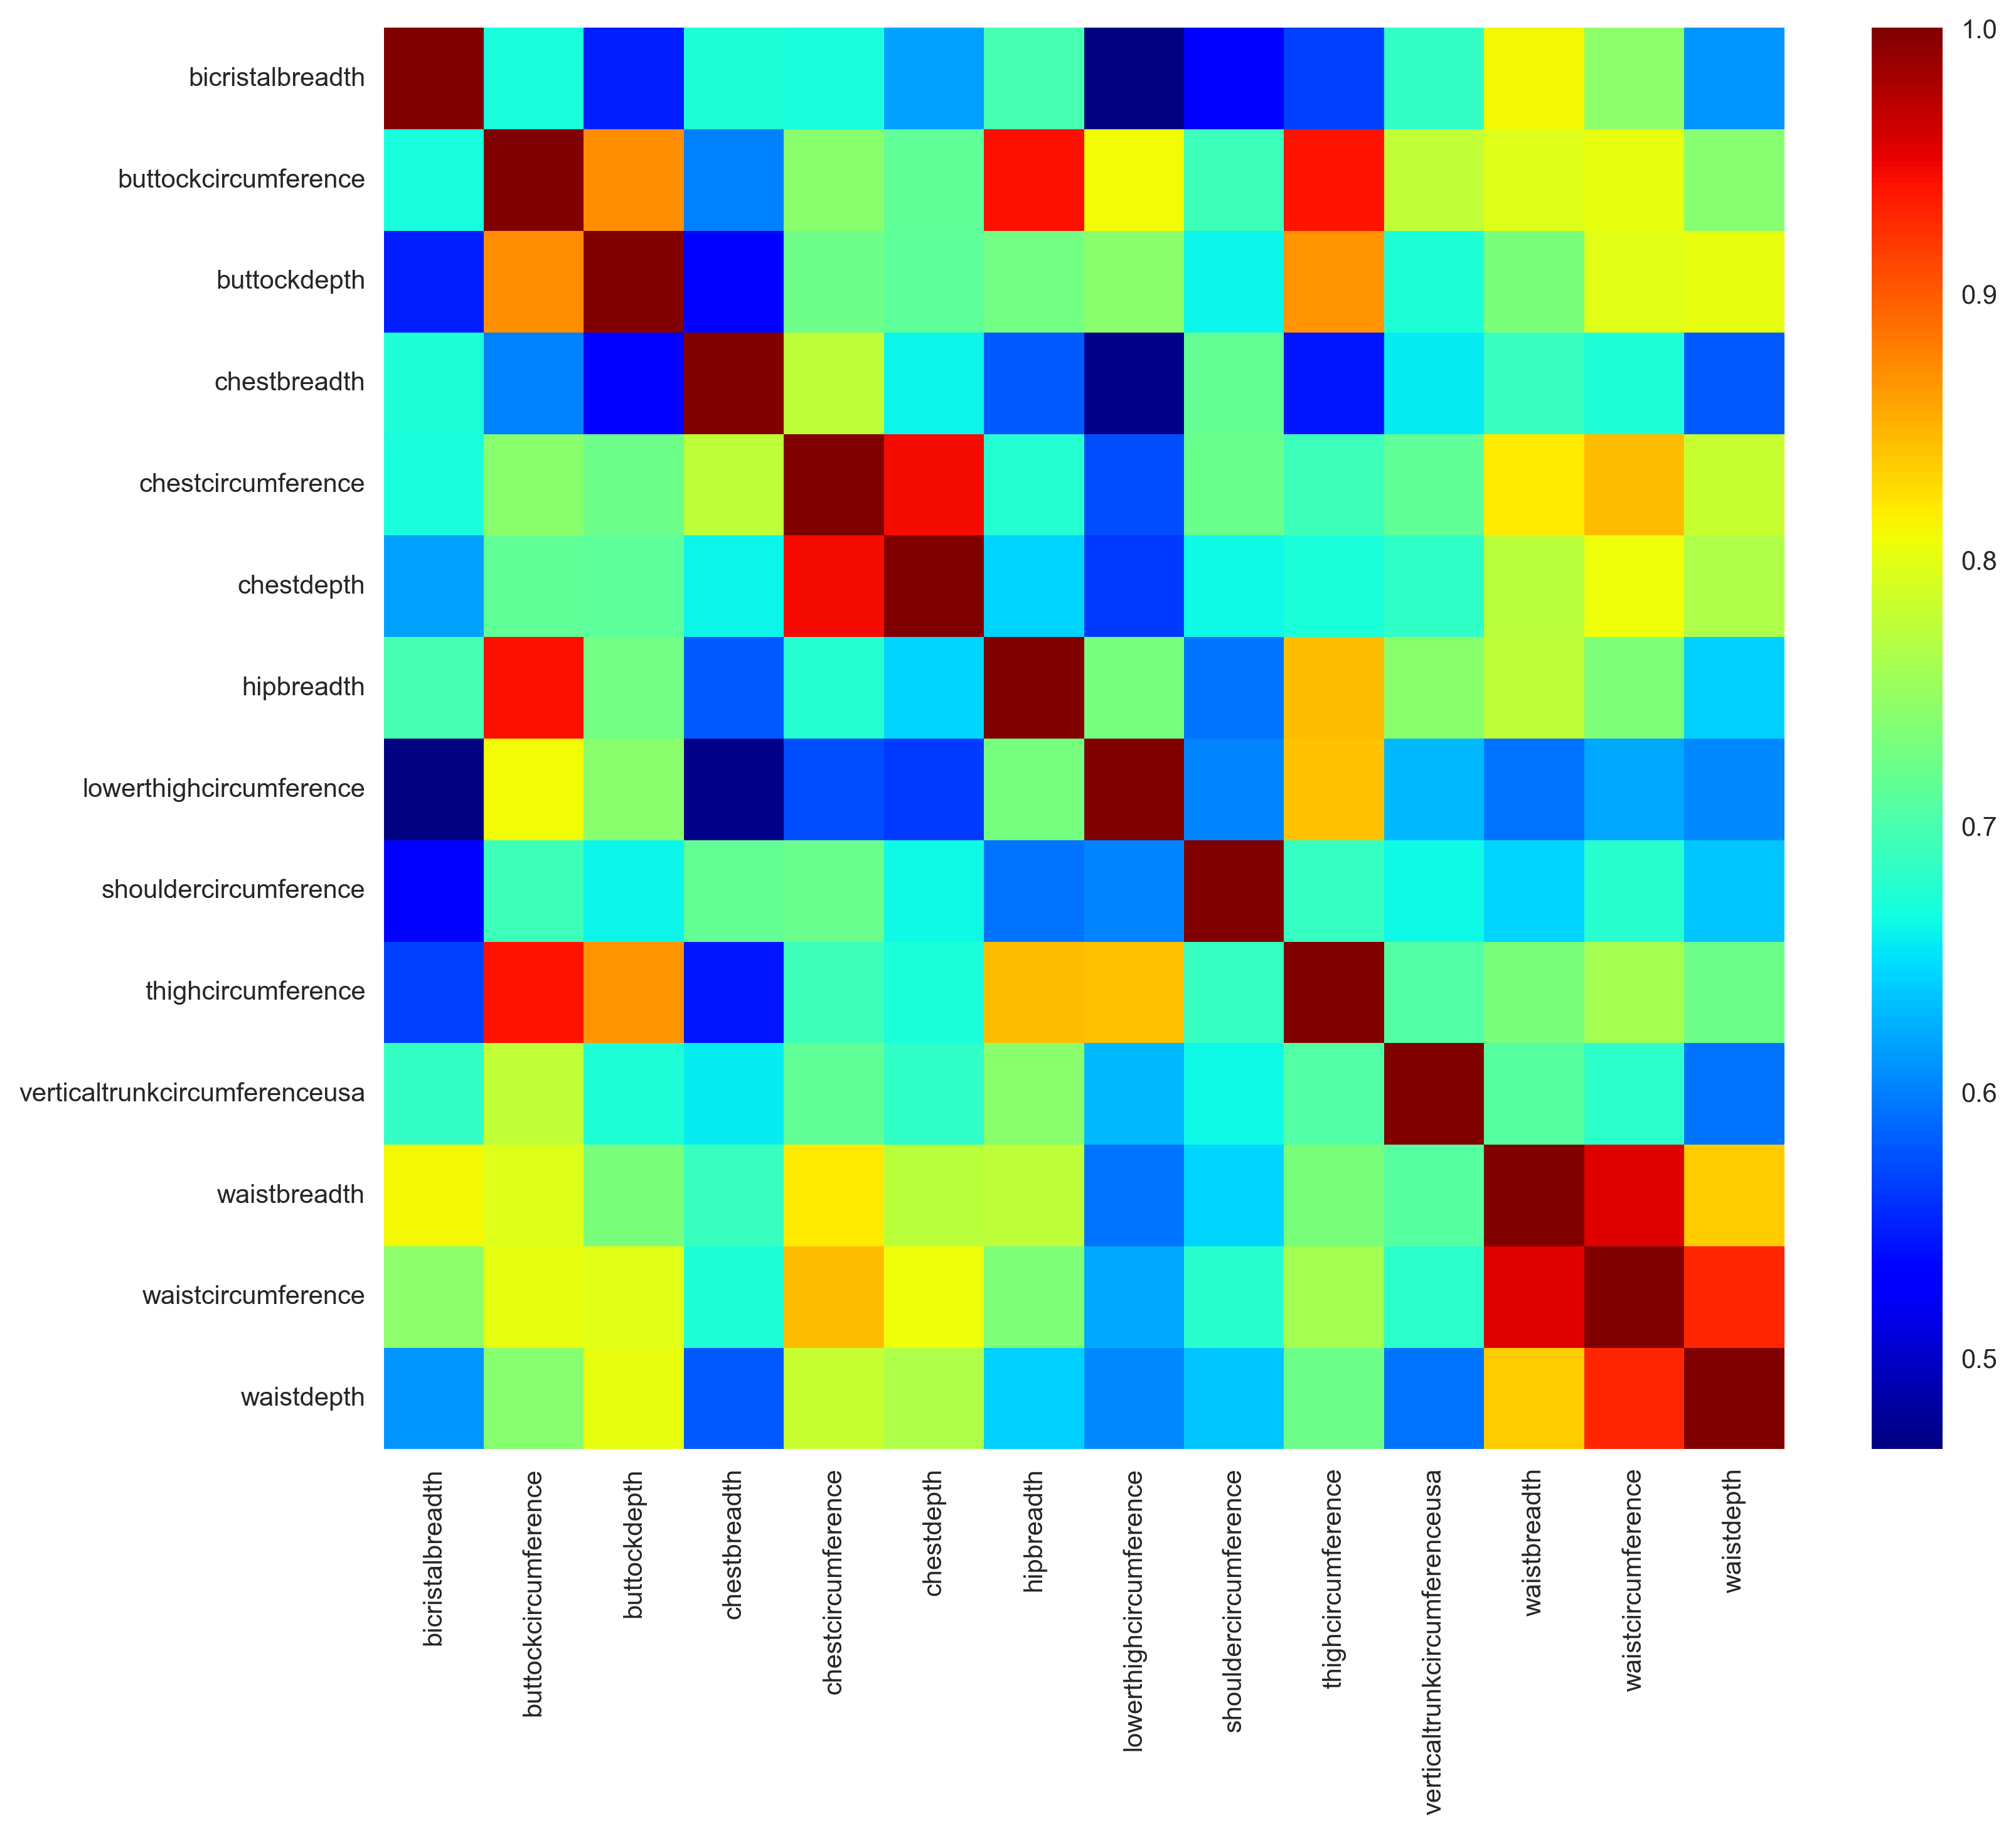
\includegraphics[width=0.75\textwidth]{../Images/FCorr.png}
\end{figure}

\subsection{Elbow method}
To calculate the optimal number of clusters, we use the python function \\
\texttt{yellowbrick.cluster.KElbowVisualizer}.
\subsubsection{K-Medoids}
\begin{figure}[H]
	\centering
	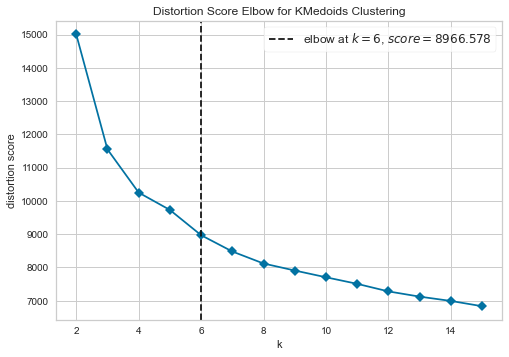
\includegraphics[width=0.5\textwidth]{../Images/FMedoidsElbow.png}
\end{figure}
We choose a number of clusters $k=6$ for the K-Medoids.

\subsubsection{Ward's Method}
\begin{figure}[H]
	\centering
	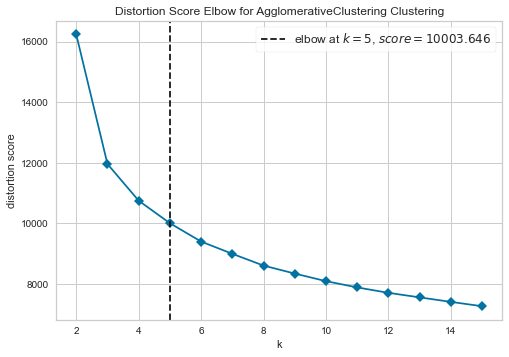
\includegraphics[width=0.5\textwidth]{../Images/FHierElbow.png}
\end{figure}
We choose a number of clusters $k=5$ for the Ward's method.

\subsection{Visualisation}
To visualise the clusters we make a projection on the plane formed by the first 2 axes of the principal component analysis (PCA).
\subsubsection{K-Medoids}
\begin{figure}[H]
	\centering
	\caption{K-Medoids Clusters}
	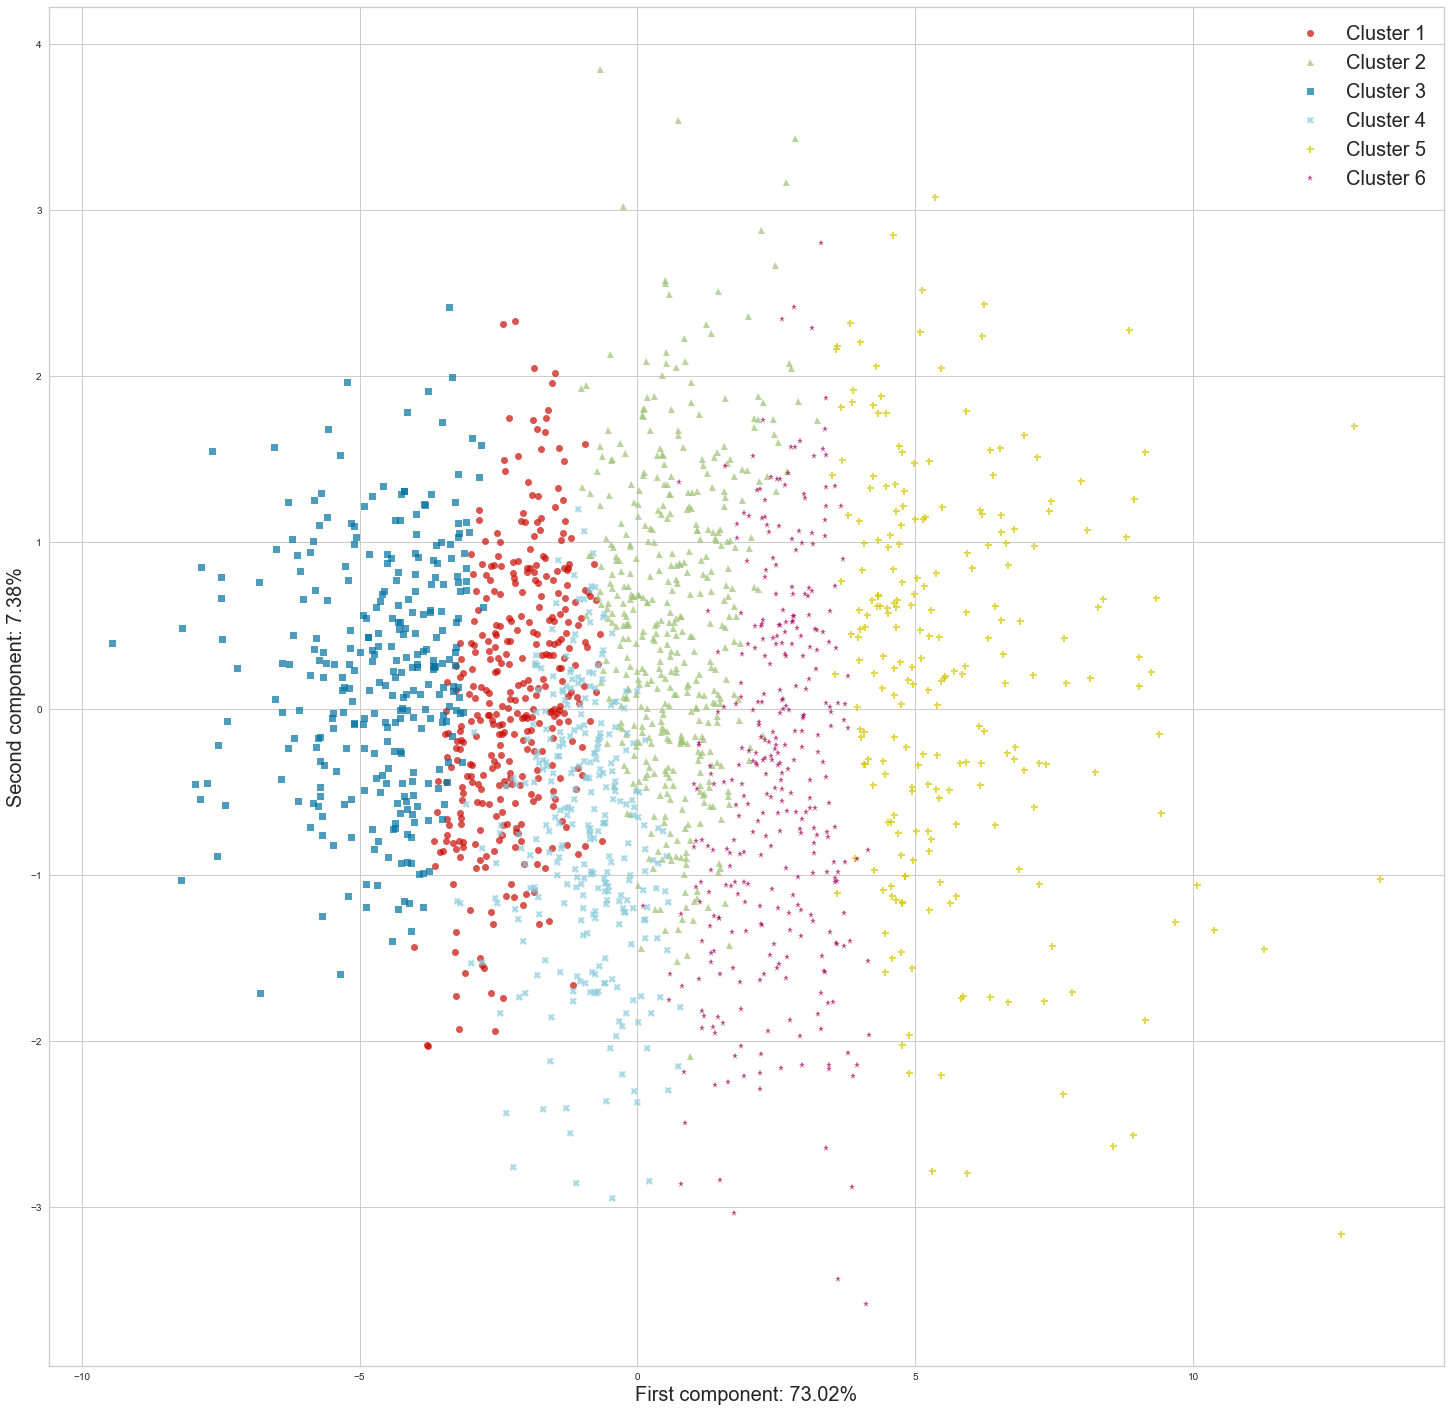
\includegraphics[width=0.7\textwidth]{../Images/FMedoidsProjection.png}
\end{figure}

\subsubsection{Ward's Method}
Here we also show a dendrogram, which is a diagram frequently used to illustrate the arrangement of groups generated by hierarchical clustering.
\begin{figure}[H]
	\centering
	\caption{Ward's Method Dendrogram}
	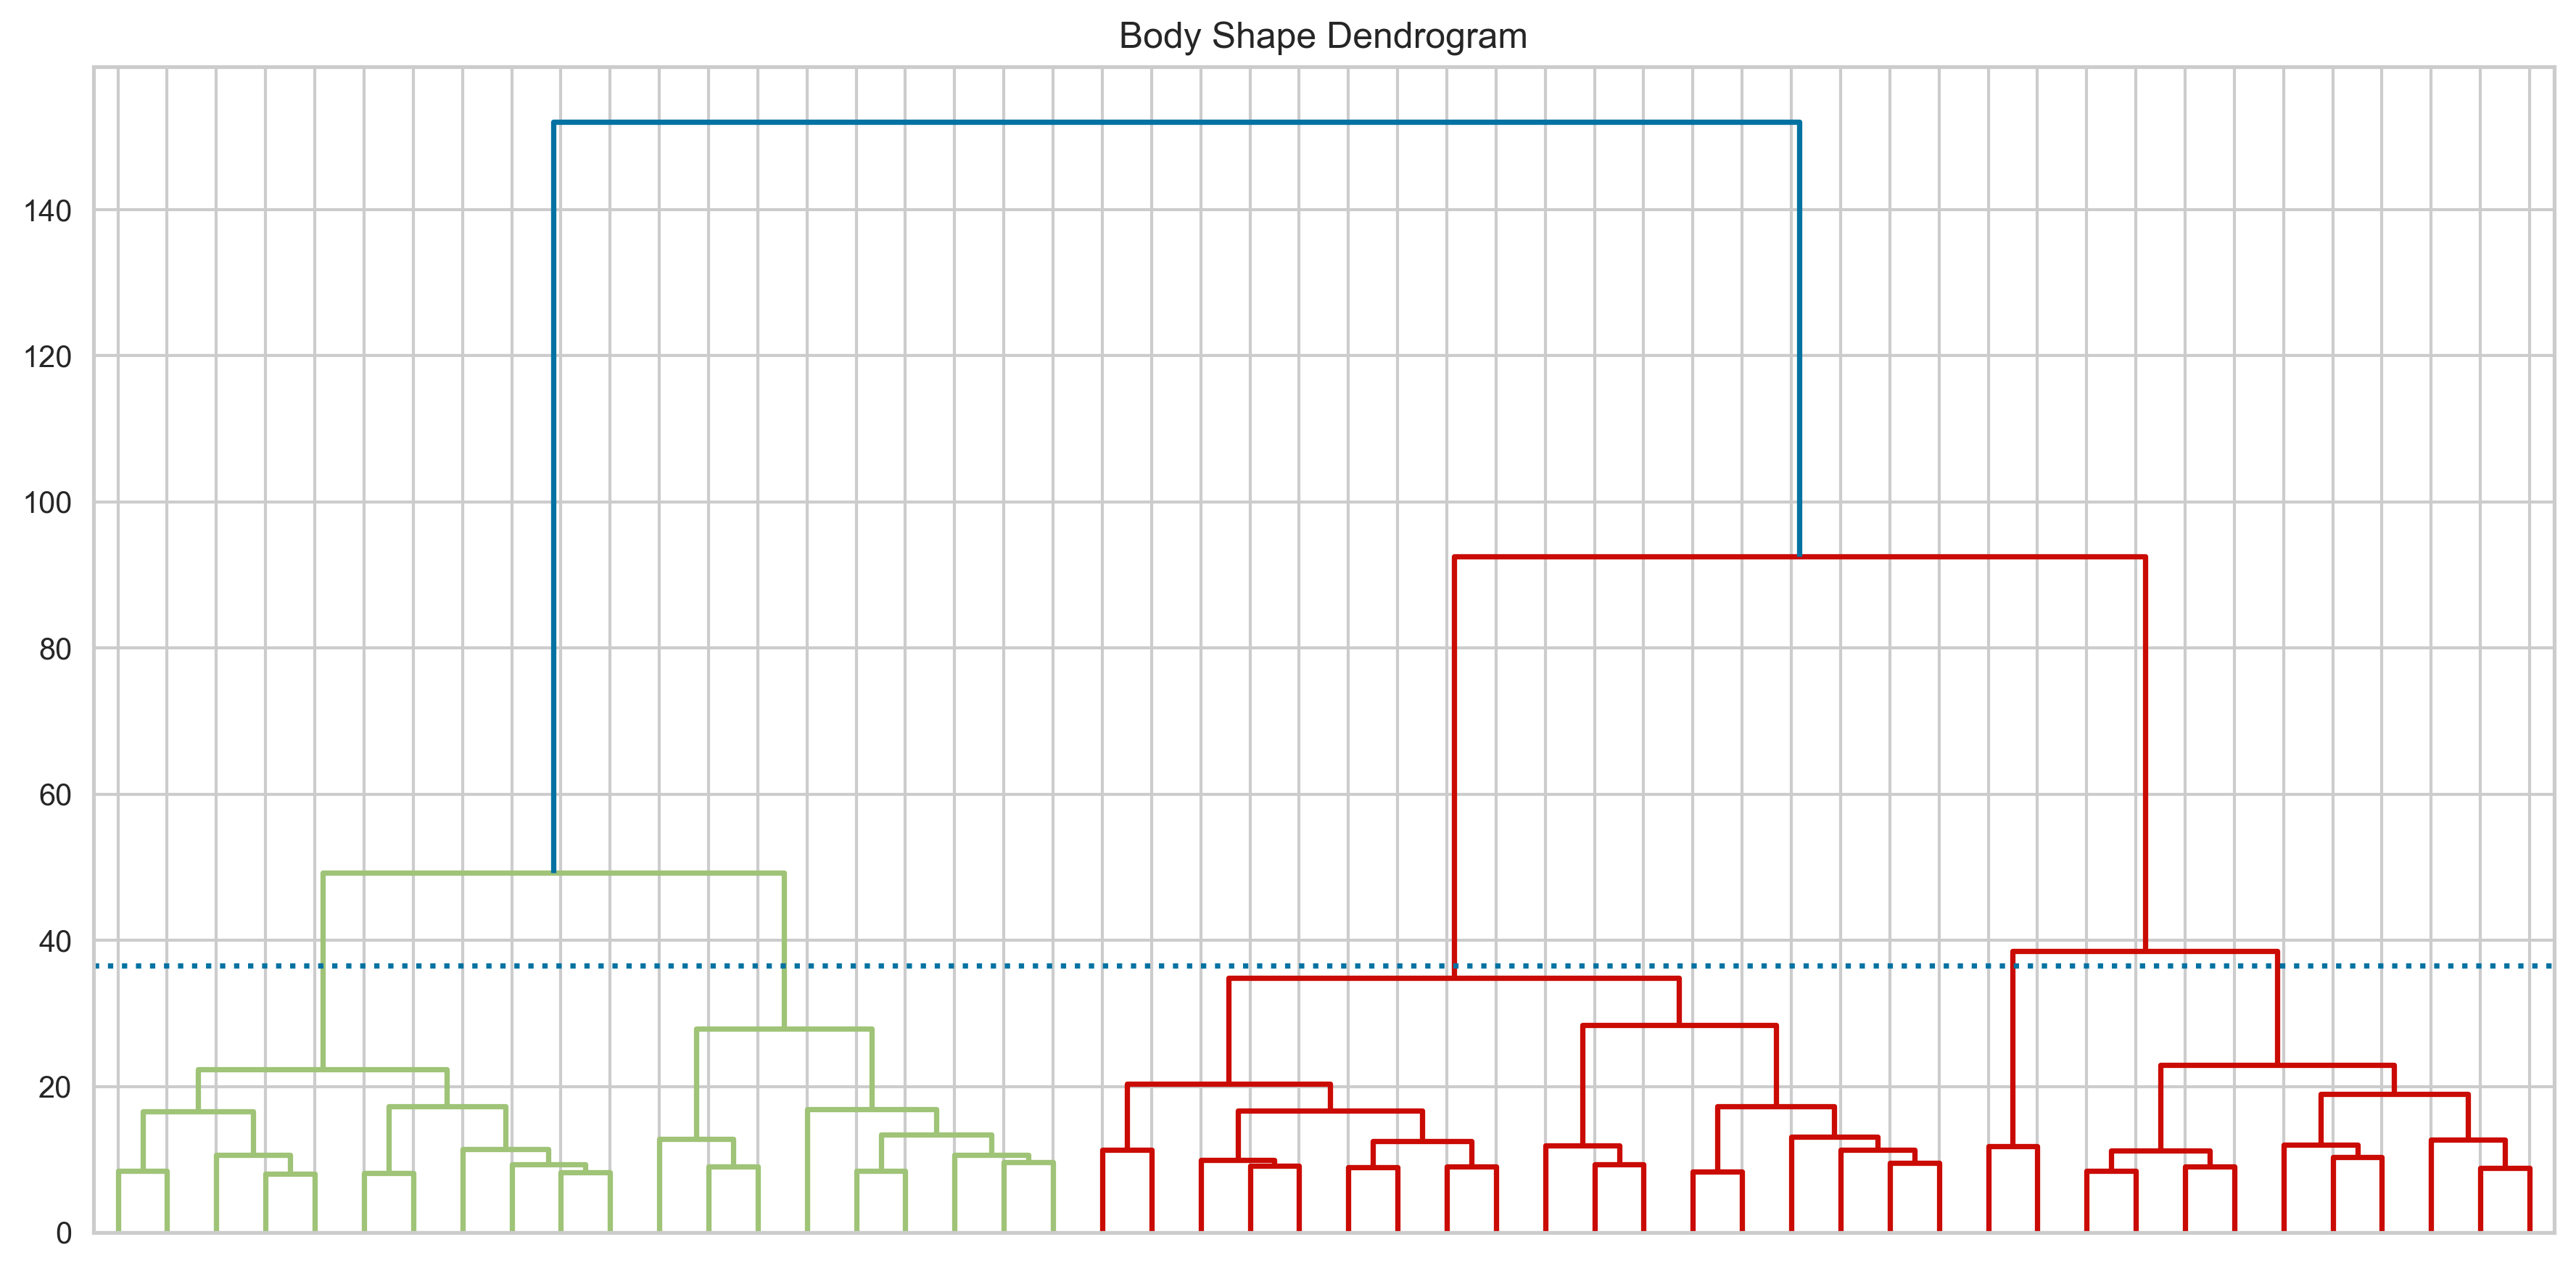
\includegraphics[width=0.7\textwidth]{../Images/FDendrogram.png}
\end{figure}

\begin{figure}[H]
	\centering
	\caption{Ward's Method Clusters}
	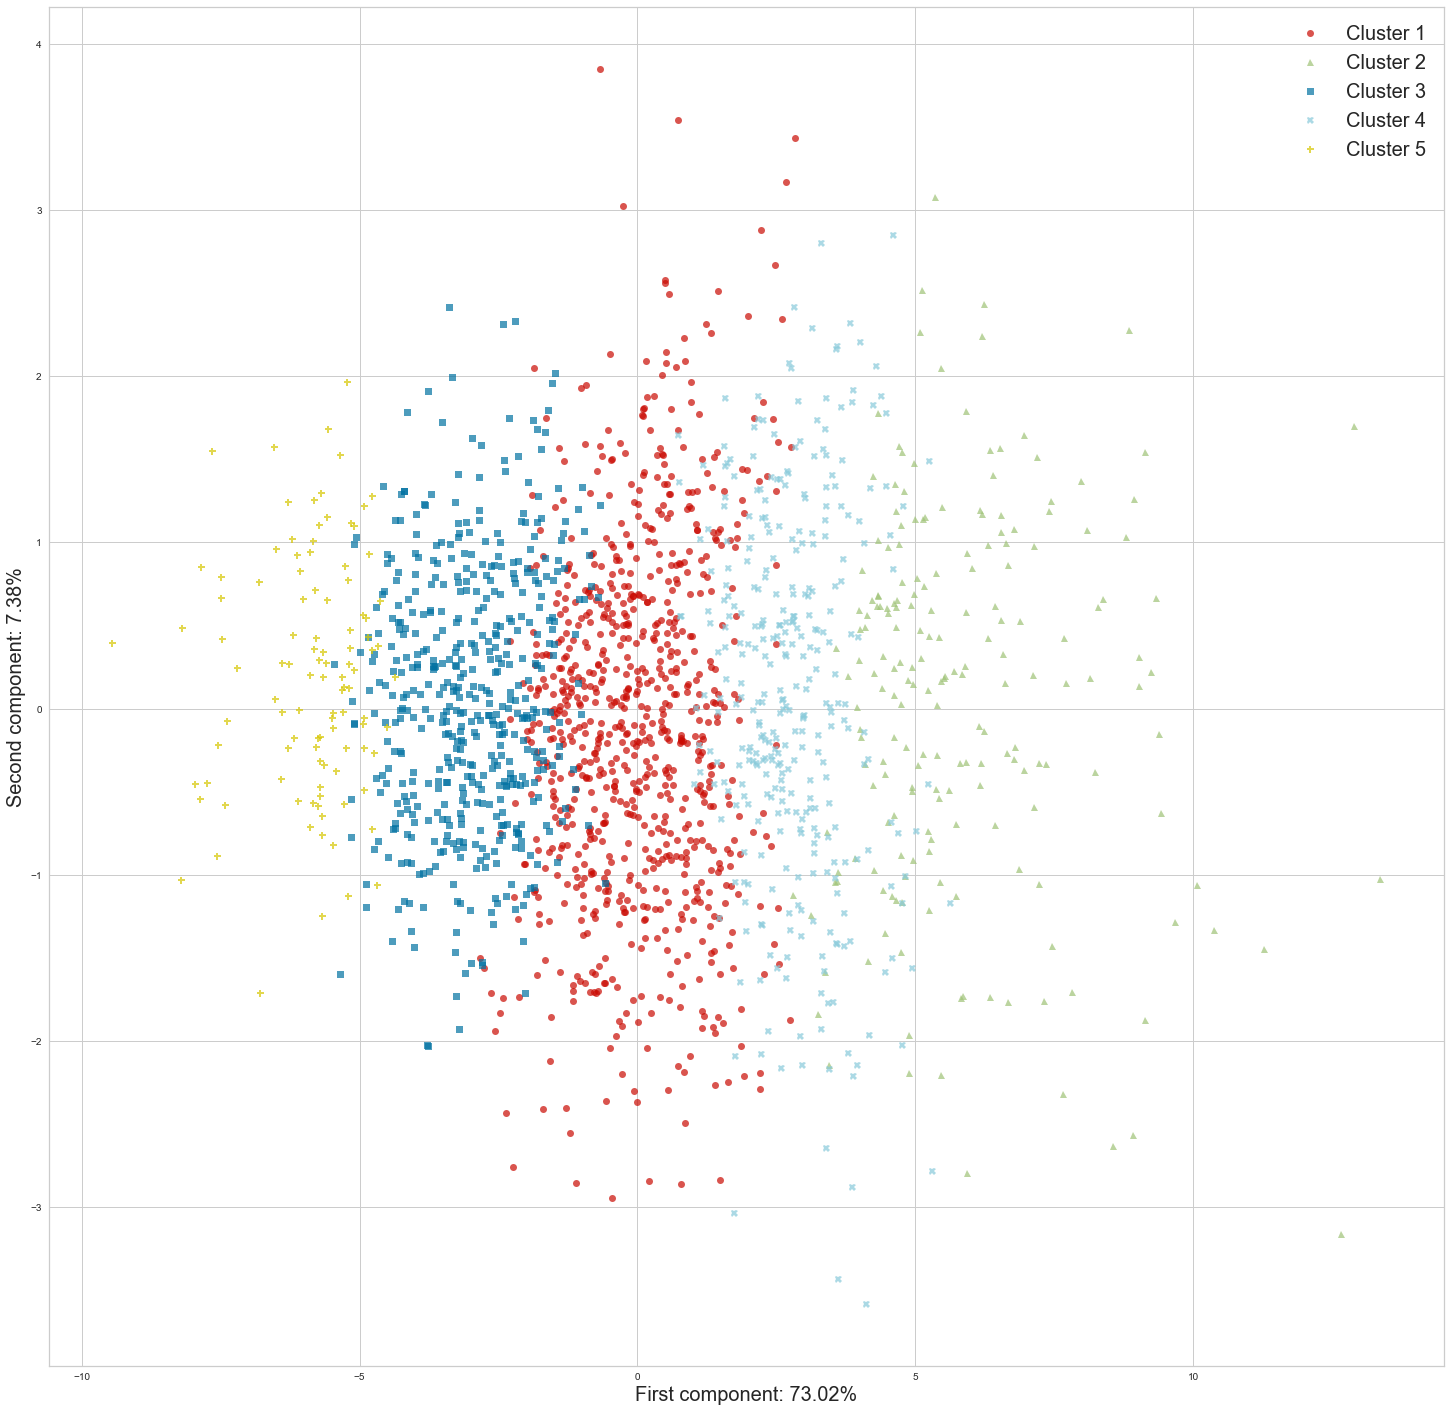
\includegraphics[width=0.7\textwidth]{../Images/FHierProjection.png}
\end{figure}

\subsection{Clusters description}
\subsubsection{K-Medoids}
\begin{table}[H]
	\footnotesize
	\centering
	\caption{Medoids}
	\begin{tabular}{lcccccc}
		\cline{2-7}
		                             & \multicolumn{6}{c}{\textbf{Cluster}}                                                                  \\
		                             & \textbf{1}                           & \textbf{2} & \textbf{3} & \textbf{4} & \textbf{5} & \textbf{6} \\
		\hline\hline
		Bicristal breadth            & 270                                  & 278        & 261        & 260        & 299        & 292        \\
		Buttock circumference        & 970                                  & 1016       & 917        & 1015       & 1136       & 1076       \\
		Buttock depth                & 216                                  & 235        & 193        & 233        & 280        & 251        \\
		Chest breadth                & 258                                  & 281        & 248        & 255        & 295        & 270        \\
		Chest circumference          & 892                                  & 962        & 866        & 906        & 1069       & 998        \\
		Chest depth                  & 227                                  & 253        & 225        & 237        & 287        & 267        \\
		Hip breadth                  & 340                                  & 357        & 322        & 344        & 387        & 366        \\
		Lower thigh circumference    & 395                                  & 402        & 351        & 398        & 443        & 534        \\
		Shoulder circumference       & 993                                  & 1035       & 965        & 1035       & 1075       & 1035       \\
		Thigh circumference          & 588                                  & 623        & 545        & 606        & 702        & 663        \\
		Vertical trunk circumference & 1519                                 & 1581       & 1477       & 1553       & 1639       & 1594       \\
		Waist breadth                & 272                                  & 316        & 268        & 276        & 357        & 324        \\
		Waist circumference          & 807                                  & 886        & 731        & 824        & 1028       & 933        \\
		Waist depth                  & 203                                  & 212        & 176        & 199        & 269        & 232        \\
		\hline
		Height (cm)                  & 160.02                               & 167.64     & 160.02     & 170.18     & 165.10     & 162.56     \\
		Weight (kg)                  & 63.50                                & 65.32      & 56.70      & 70.31      & 81.65      & 73.94      \\
		BMI                          & 24.80                                & 23.24      & 22.14      & 24.28      & 29.95      & 27.98
	\end{tabular}
\end{table}

\begin{table}[H]
	\footnotesize
	\centering
	\caption{Means}
	\begin{tabular}{lcccccc}
		\cline{2-7}
		                             & \multicolumn{6}{c}{\textbf{Cluster}}                                                                            \\
		                             & \textbf{1}                           & \textbf{2}   & \textbf{3}   & \textbf{4}   & \textbf{5}   & \textbf{6}   \\
		\hline\hline
		Bicristal breadth            & 264.87                               & 279.85       & 250.56       & 257.97       & 304.40       & 285.79       \\
		Buttock circumference        & 971.19                               & 1025.85      & 913.16       & 1015.66      & 1140.41      & 1086.44      \\
		Buttock depth                & 215.91                               & 231.80       & 201.88       & 233.22       & 271.63       & 252.97       \\
		Chest breadth                & 260.40                               & 278.94       & 248.44       & 259.82       & 294.71       & 275.44       \\
		Chest circumference          & 892.16                               & 972.16       & 845.13       & 913.87       & 1084.39      & 995.67       \\
		Chest depth                  & 229.04                               & 254.31       & 215.36       & 239.00       & 290.64       & 263.69       \\
		Hip breadth                  & 338.80                               & 357.38       & 318.61       & 349.07       & 391.98       & 374.09       \\
		Lower thigh circumference    & 383.46                               & 399.40       & 357.00       & 402.33       & 446.39       & 426.38       \\
		Shoulder circumference       & 995.66                               & 1040.72      & 962.36       & 1027.85      & 1102.64      & 1053.20      \\
		Thigh circumference          & 581.25                               & 617.04       & 538.02       & 616.74       & 698.05       & 663.93       \\
		Vertical trunk circumference & 1512.24                              & 1576.08      & 1469.05      & 1542.88      & 1667.78      & 1607.07      \\
		Waist breadth                & 281.69                               & 308.71       & 257.91       & 282.77       & 354.14       & 322.38       \\
		Waist circumference          & 801.46                               & 881.72       & 730.60       & 817.72       & 1031.28      & 932.32       \\
		Waist depth                  & 194.05                               & 215.56       & 177.07       & 202.71       & 265.71       & 234.44       \\
		\hline
		Age                          & 26.64                                & 29.04        & 26.67        & 27.81        & 33.14        & 31.38        \\
		Height (cm)                  & 161.81                               & 164.86       & 160.23       & 164.78       & 168.53       & 166.29       \\
		Weight (kg)                  & 59.84                                & 67.86        & 53.18        & 65.50        & 81.79        & 74.39        \\
		BMI                          & 22.90                                & 25.02        & 20.75        & 24.20        & 29.82        & 27.30        \\
		\hline
		\textit{Count}               & \textit{360}                         & \textit{452} & \textit{299} & \textit{301} & \textit{232} & \textit{342}
	\end{tabular}
\end{table}

\subsubsection{Ward's Method}
\begin{table}[H]
	\footnotesize
	\centering
	\caption{Medoids}
	\begin{tabular}{lccccc}
		\cline{2-6}
		                             & \multicolumn{5}{c}{\textbf{Cluster}}                                                     \\
		                             & \textbf{1}                           & \textbf{2} & \textbf{3} & \textbf{4} & \textbf{5} \\
		\hline\hline
		Bicristal breadth            & 271                                  & 299        & 253        & 292        & 232        \\
		Buttock circumference        & 1011                                 & 1136       & 981        & 1076       & 876        \\
		Buttock depth                & 236                                  & 280        & 217        & 251        & 201        \\
		Chest breadth                & 274                                  & 295        & 251        & 270        & 241        \\
		Chest circumference          & 926                                  & 1069       & 872        & 998        & 808        \\
		Chest depth                  & 245                                  & 287        & 221        & 267        & 199        \\
		Hip breadth                  & 346                                  & 387        & 328        & 366        & 306        \\
		Lower thigh circumference    & 408                                  & 443        & 375        & 435        & 360        \\
		Shoulder circumference       & 1013                                 & 1075       & 990        & 1035       & 934        \\
		Thigh circumference          & 635                                  & 702        & 576        & 663        & 510        \\
		Vertical trunk circumference & 1604                                 & 1639       & 1526       & 1594       & 1411       \\
		Waist breadth                & 288                                  & 357        & 273        & 324        & 241        \\
		Waist circumference          & 847                                  & 1028       & 751        & 933        & 694        \\
		Waist depth                  & 213                                  & 269        & 180        & 232        & 168        \\
		\hline
		Height (cm)                  & 162.56                               & 165.10     & 165.10     & 162.56     & 147.32     \\
		Weight (kg)                  & 68.04                                & 81.65      & 58.06      & 73.94      & 46.72      \\
		BMI                          & 24.96                                & 29.95      & 21.30      & 27.98      & 21.53      \\
	\end{tabular}
\end{table}

\begin{table}[H]
	\footnotesize
	\centering
	\caption{Means}
	\begin{tabular}{lccccc}
		\cline{2-6}
		                             & \multicolumn{5}{c}{\textbf{Cluster}}                                                             \\
		                             & \textbf{1}                           & \textbf{2}   & \textbf{3}   & \textbf{4}   & \textbf{5}   \\
		\hline\hline
		Bicristal breadth            & 272.00                               & 304.44       & 258.05       & 290.10       & 241.75       \\
		Buttock circumference        & 1023.85                              & 1145.92      & 953.31       & 1083.18      & 883.93       \\
		Buttock depth                & 232.58                               & 274.36       & 212.08       & 251.15       & 196.41       \\
		Chest breadth                & 269.94                               & 293.10       & 256.20       & 281.37       & 242.37       \\
		Chest circumference          & 943.96                               & 1084.66      & 878.83       & 1011.03      & 821.18       \\
		Chest depth                  & 246.12                               & 292.01       & 226.07       & 267.25       & 209.18       \\
		Hip breadth                  & 355.12                               & 393.09       & 332.02       & 373.99       & 306.83       \\
		Lower thigh circumference    & 403.12                               & 449.87       & 374.27       & 420.94       & 347.40       \\
		Shoulder circumference       & 1029.85                              & 1107.76      & 989.31       & 1062.31      & 942.58       \\
		Thigh circumference          & 618.78                               & 703.84       & 568.17       & 658.48       & 518.18       \\
		Vertical trunk circumference & 1558.54                              & 1669.85      & 1502.72      & 1615.76      & 1441.26      \\
		Waist breadth                & 298.75                               & 355.29       & 272.37       & 327.45       & 244.24       \\
		Waist circumference          & 856.81                               & 1036.32      & 773.93       & 945.45       & 696.40       \\
		Waist depth                  & 210.79                               & 268.05       & 187.36       & 236.94       & 169.92       \\
		\hline
		Age                          & 28.71                                & 32.90        & 26.76        & 31.36        & 25.73        \\
		Height (cm)                  & 164.20                               & 168.69       & 162,07       & 166,04       & 157.72       \\
		Weight (kg)                  & 66.66                                & 85.16        & 58.00        & 75.04        & 49.88        \\
		BMI                          & 24.78                                & 30.00        & 22.13        & 27.26        & 20.09        \\
		\hline
		\textit{Count}               & \textit{831}                         & \textit{200} & \textit{503} & \textit{347} & \textit{105}
	\end{tabular}
\end{table}

\section{Male data set}
\vspace{-8mm}
\begin{table}[H]
	\caption{Male data set}
	\centering
	\begin{tabular}{|cccc|c|}
		\hline
		Age   & Height (cm) & Weight (kg) & BMI   & \textit{Count} \\
		\hline
		30.16 & 177.89      & 85.28       & 26.93 & \textit{4082}  \\
		\hline
	\end{tabular}
\end{table}

\subsection{Correlation matrix}
We calculate the correlation matrix of the measurements.
\begin{figure}[H]
	\centering
	\caption{Correlation matrix for the male data set}
	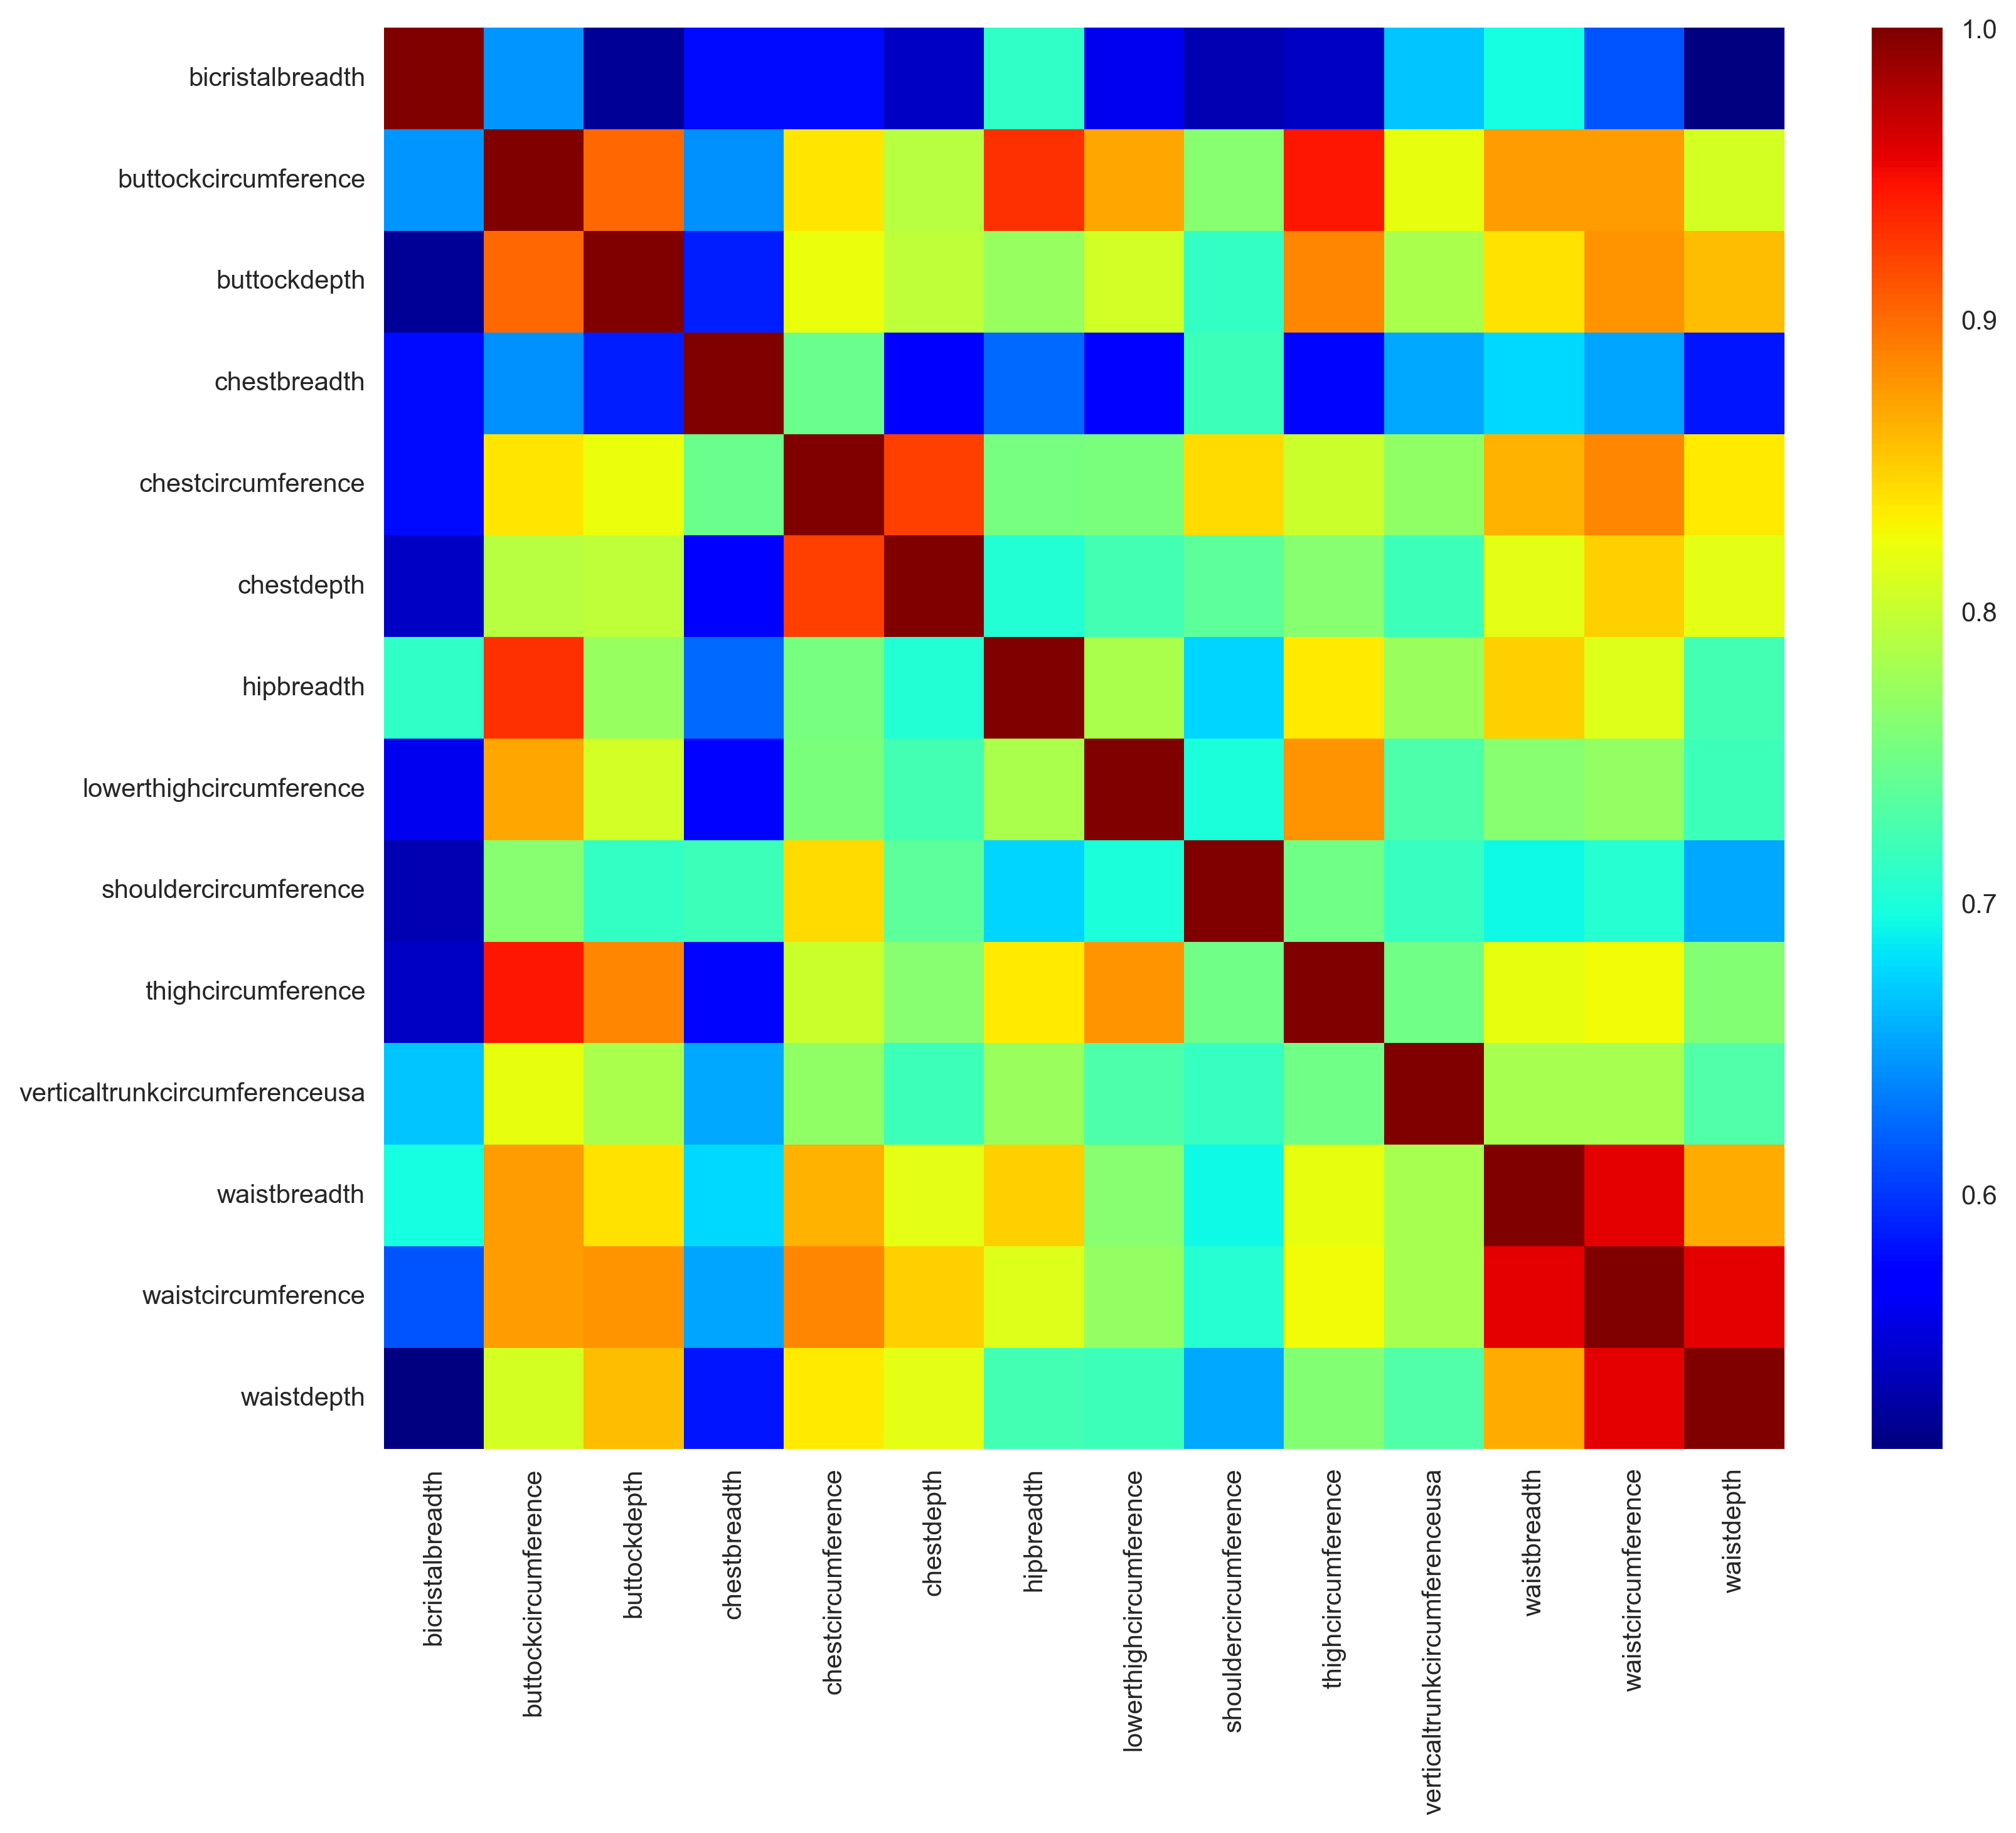
\includegraphics[width=0.7\textwidth]{../Images/MCorr.png}
\end{figure}

\subsection{Elbow method}
To calculate the optimal number of clusters, we use the python function \\
\texttt{yellowbrick.cluster.KElbowVisualizer}.
\subsubsection{K-Medoids}
\begin{figure}[H]
	\centering
	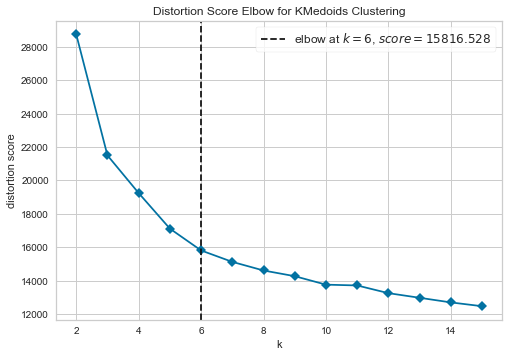
\includegraphics[width=0.5\textwidth]{../Images/MMedoidsElbow.png}
\end{figure}
We choose a number of clusters $k=6$ for the K-Medoids.

\subsubsection{Ward's Method}
\begin{figure}[H]
	\centering
	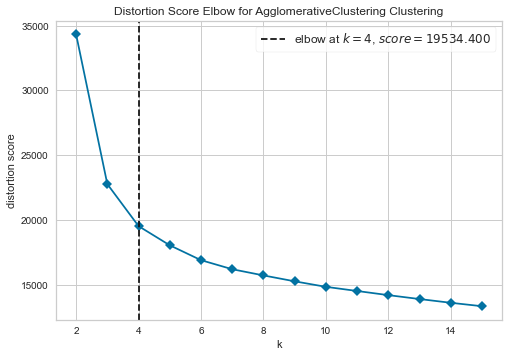
\includegraphics[width=0.5\textwidth]{../Images/MHierElbow.png}
\end{figure}
We choose a number of clusters $k=4$ for the Ward's method.

\subsection{Visualisation}
To visualise the clusters we make a projection on the plane formed by the first 2 axes of the principal component analysis (PCA).
\subsubsection{K-Medoids}
\begin{figure}[H]
	\centering
	\caption{K-Medoids Clusters}
	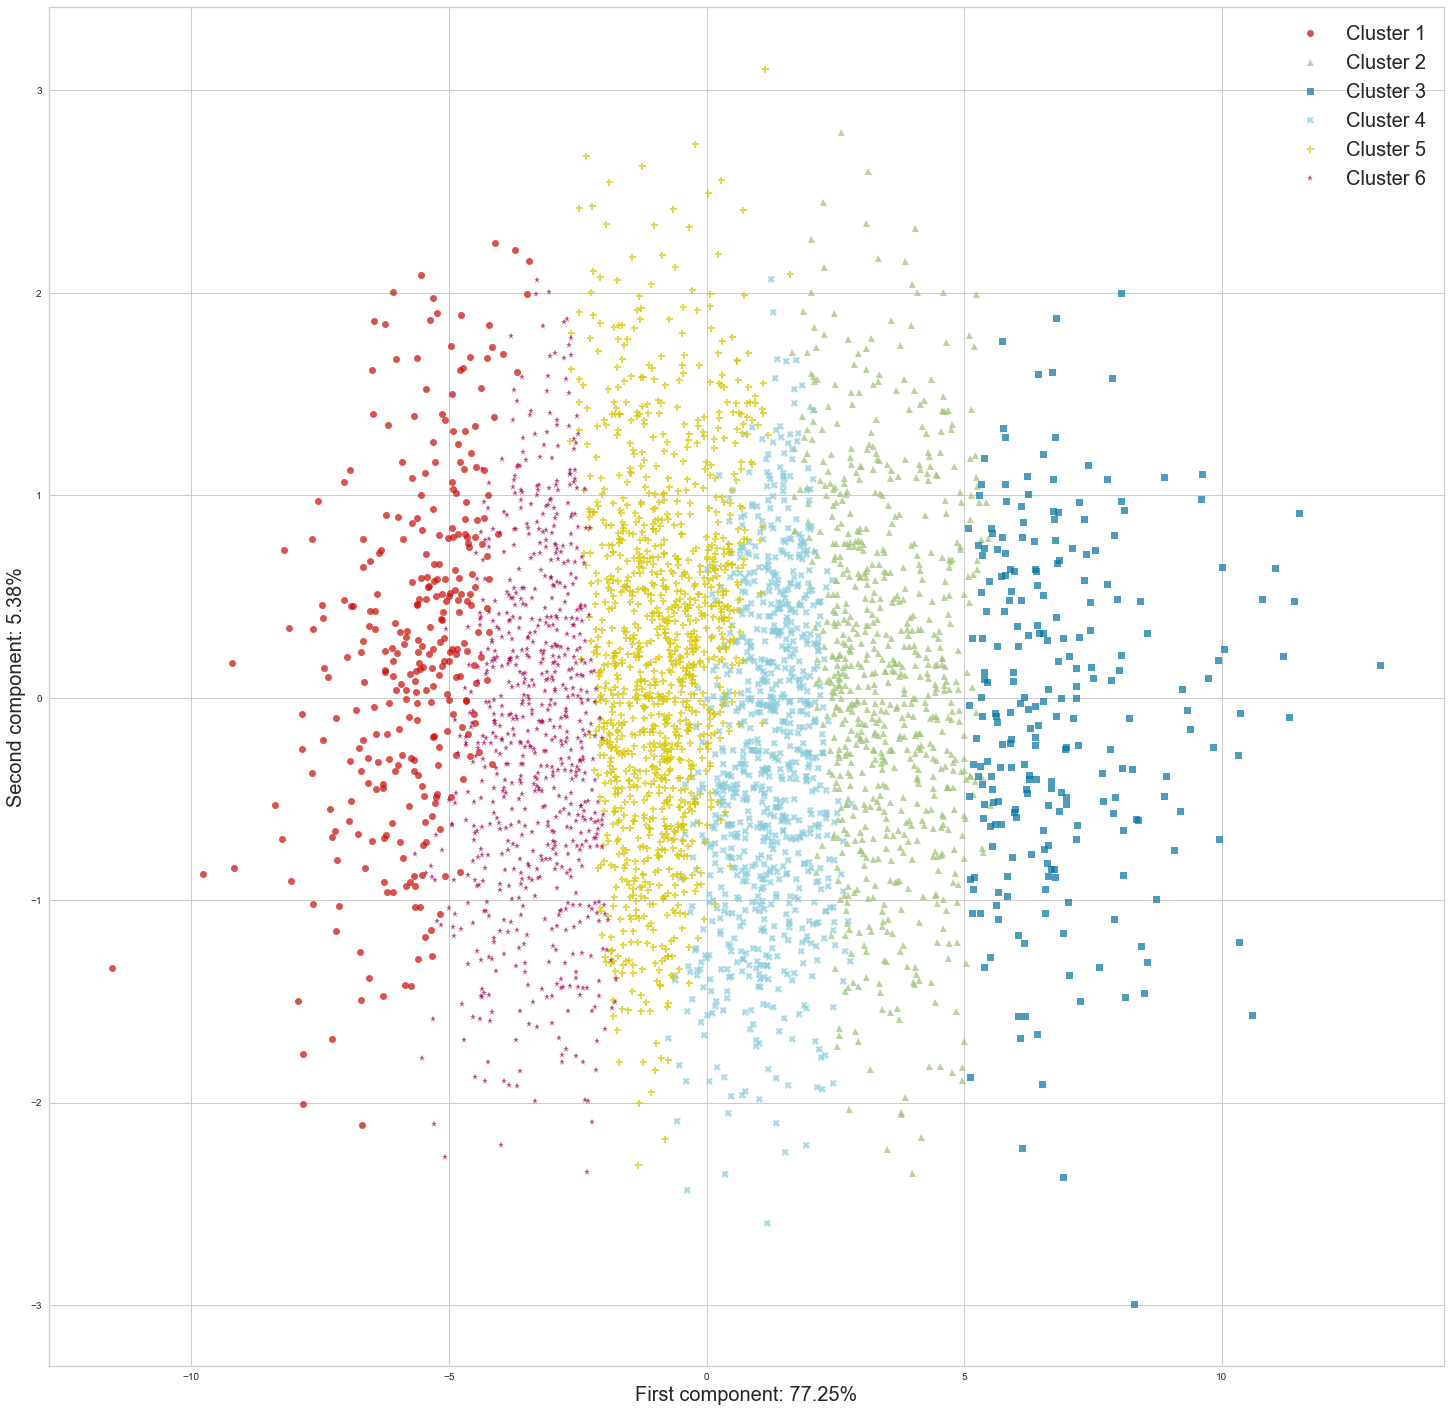
\includegraphics[width=0.7\textwidth]{../Images/MMedoidsProjection.png}
\end{figure}

\subsubsection{Ward's Method}
Here we also show a dendrogram.
\begin{figure}[H]
	\centering
	\caption{Ward's Method Dendrogram}
	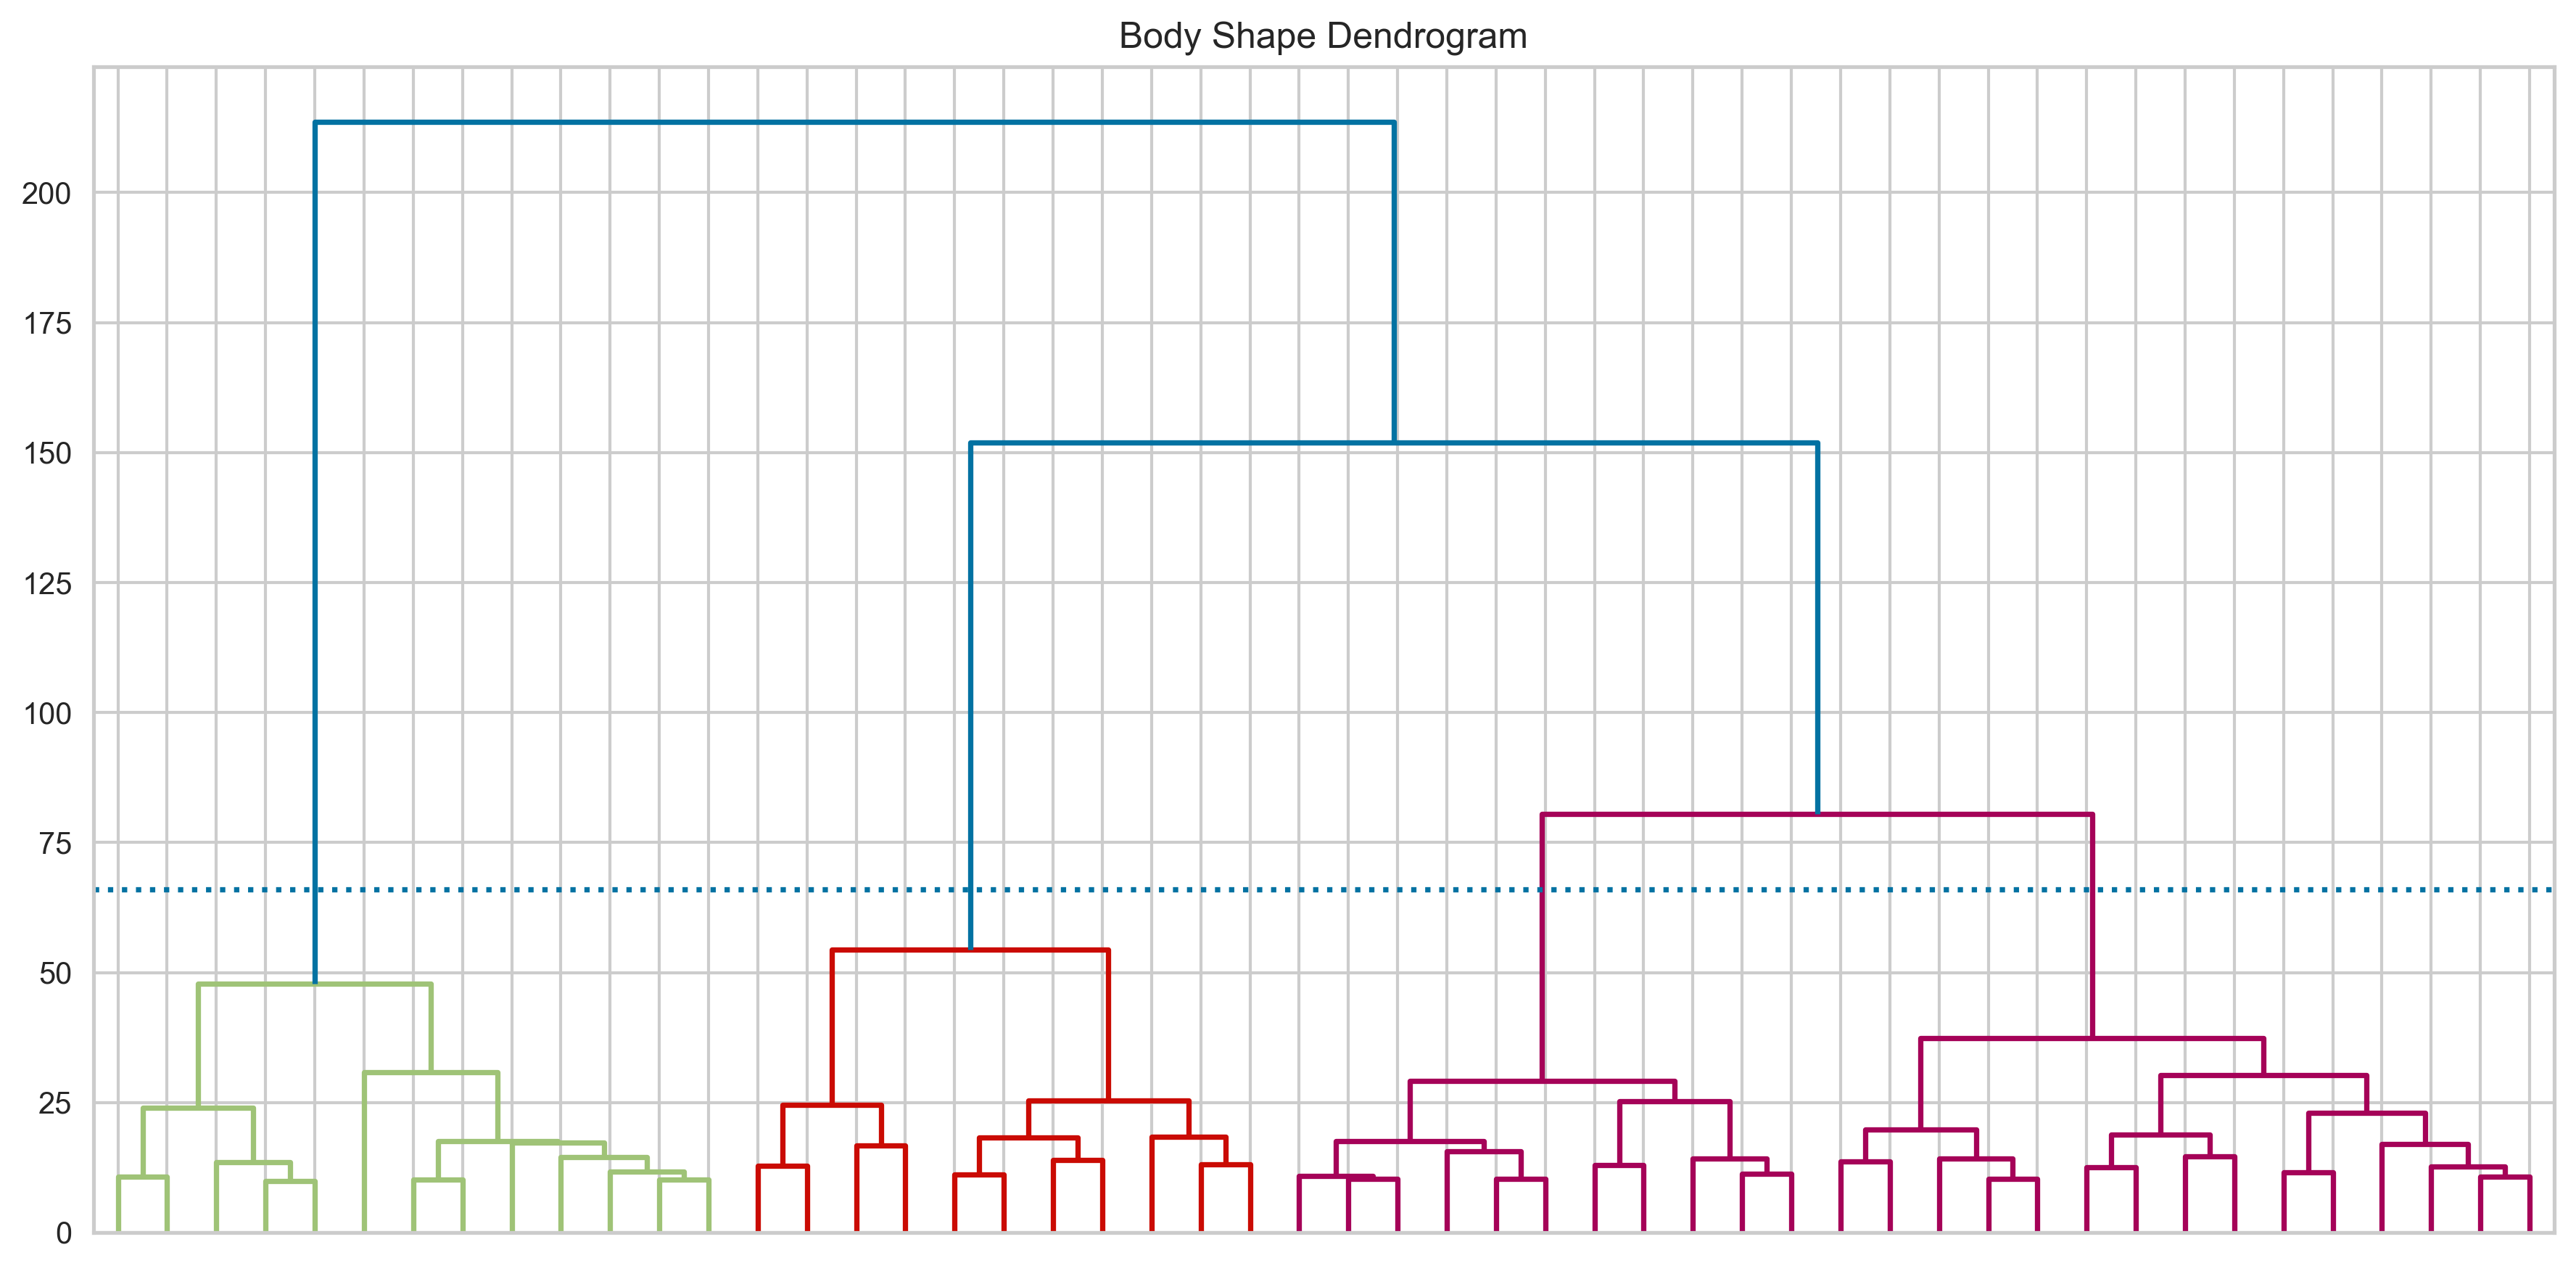
\includegraphics[width=0.7\textwidth]{../Images/MDendrogram.png}
\end{figure}

\begin{figure}[H]
	\centering
	\caption{Ward's Method Clusters}
	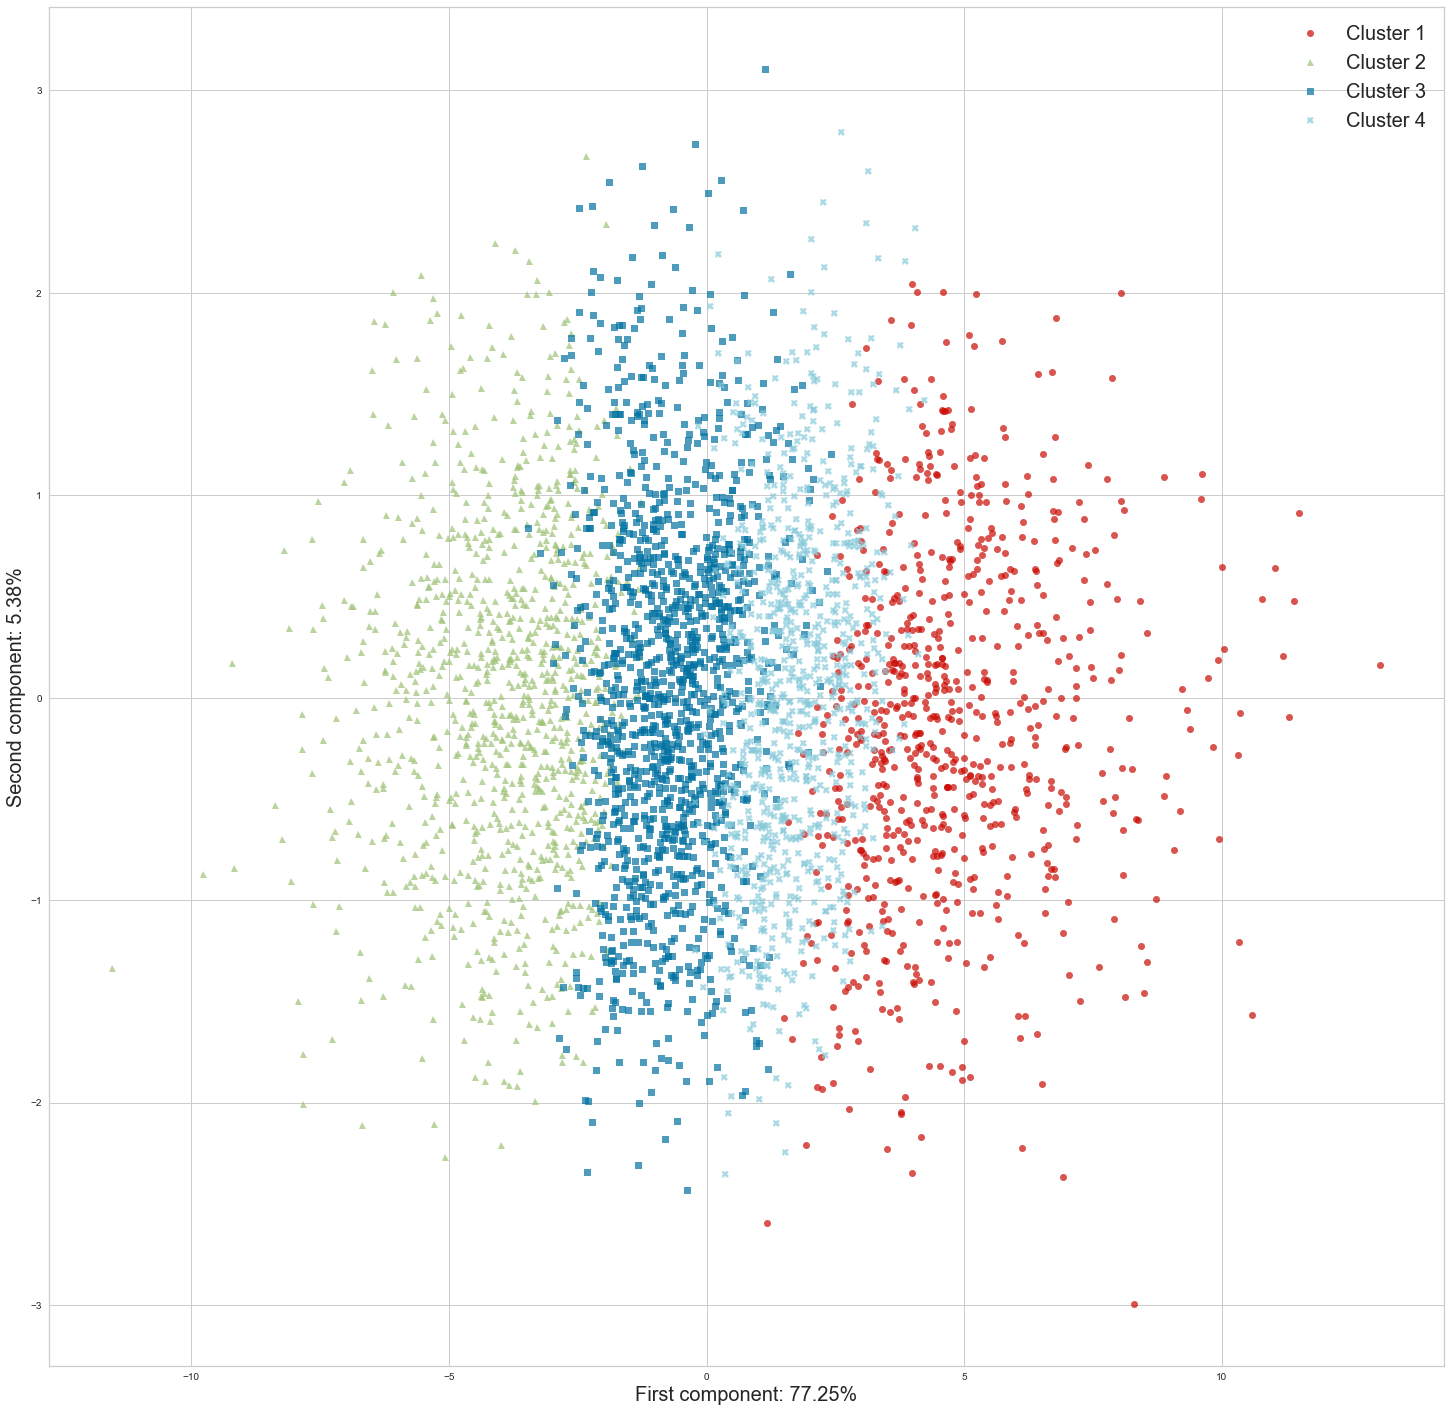
\includegraphics[width=0.7\textwidth]{../Images/MHierProjection.png}
\end{figure}

\subsection{Clusters description}
\subsubsection{K-Medoids}
\begin{table}[H]
	\footnotesize
	\centering
	\caption{Medoids}
	\begin{tabular}{lcccccc}
		\cline{2-7}
		                             & \multicolumn{6}{c}{\textbf{Cluster}}                                                                  \\
		                             & \textbf{1}                           & \textbf{2} & \textbf{3} & \textbf{4} & \textbf{5} & \textbf{6} \\
		\hline\hline
		Bicristal breadth            & 275                                  & 252        & 263        & 293        & 301        & 269        \\
		Buttock circumference        & 1004                                 & 1073       & 916        & 1097       & 1178       & 959        \\
		Buttock depth                & 242                                  & 251        & 214        & 267        & 293        & 220        \\
		Chest breadth                & 288                                  & 298        & 263        & 300        & 316        & 278        \\
		Chest circumference          & 1026                                 & 1100       & 940        & 1145       & 1237       & 996        \\
		Chest depth                  & 241                                  & 266        & 224        & 276        & 304        & 238        \\
		Hip breadth                  & 345                                  & 362        & 317        & 373        & 396        & 331        \\
		Lower thigh circumference    & 403                                  & 437        & 376        & 443        & 460        & 379        \\
		Shoulder circumference       & 1173                                 & 1190       & 1082       & 1245       & 1255       & 1140       \\
		Thigh circumference          & 613                                  & 653        & 553        & 679        & 730        & 587        \\
		Vertical trunk circumference & 1657                                 & 1682       & 1559       & 1742       & 1813       & 1604       \\
		Waist breadth                & 322                                  & 362        & 285        & 367        & 402        & 308        \\
		Waist circumference          & 902                                  & 1012       & 784        & 1078       & 1167       & 860        \\
		Waist depth                  & 220                                  & 255        & 199        & 270        & 306        & 212        \\
		\hline
		Height (cm)                  & 175.26                               & 185.42     & 172.72     & 177.80     & 175.26     & 170.18     \\
		Weight (kg)                  & 79.38                                & 96.62      & 70.31      & 97.52      & 79.38      & 67.13      \\
		BMI                          & 25.84                                & 28.10      & 23.56      & 30.85      & 33.75      & 24.75
	\end{tabular}
\end{table}

\begin{table}[H]
	\footnotesize
	\centering
	\caption{Means}
	\begin{tabular}{lcccccc}
		\cline{2-7}
		                             & \multicolumn{6}{c}{\textbf{Cluster}}                                                                             \\
		                             & \textbf{1}                           & \textbf{2}   & \textbf{3}   & \textbf{4}   & \textbf{5}    & \textbf{6}   \\
		\hline\hline
		Bicristal breadth            & 258.85                               & 289.87       & 301.60       & 276.16       & 274.10        & 260.88       \\
		Buttock circumference        & 888.46                               & 1097.33      & 1175.34      & 1042.16      & 1002.36       & 947.35       \\
		Buttock depth                & 203.21                               & 270.81       & 297.09       & 256.19       & 238.10        & 222.51       \\
		Chest breadth                & 266.54                               & 304.60       & 315.88       & 292.76       & 287.50        & 284.67       \\
		Chest circumference          & 916.22                               & 1143.49      & 1224.53      & 1096.04      & 1033.34       & 977.17       \\
		Chest depth                  & 212.10                               & 277.48       & 300.32       & 266.28       & 245.60        & 231.38       \\
		Hip breadth                  & 310.12                               & 369.20       & 392.81       & 350.47       & 341.45        & 323.36       \\
		Lower thigh circumference    & 356.46                               & 437.62       & 467.97       & 418.71       & 402.94        & 383.29       \\
		Shoulder circumference       & 1080.04                              & 1235.39      & 1284.64      & 1196.08      & 1166.80       & 1125.71      \\
		Thigh circumference          & 521.68                               & 679.03       & 737.53       & 643.89       & 613.09        & 575.66       \\
		Vertical trunk circumference & 1532.31                              & 1749.64      & 1821.66      & 1686.94      & 1650.50       & 1582.26      \\
		Waist breadth                & 272.79                               & 361.23       & 394.14       & 339.52       & 317.06        & 292.08       \\
		Waist circumference          & 764.56                               & 1051.71      & 1162.59      & 987.48       & 905.36        & 833.12       \\
		Waist depth                  & 188.54                               & 269.77       & 305.78       & 252.28       & 225.12        & 207.64       \\
		\hline
		Age                          & 30.49                                & 32.70        & 25.43        & 32.74        & 31.47         & 26.80        \\
		Height (cm)                  & 174.67                               & 180.69       & 183.11       & 177.06       & 178.46        & 174.84       \\
		Weight (kg)                  & 64.28                                & 98.97        & 113.35       & 89.00        & 81.57         & 72.89        \\
		BMI                          & 26.12                                & 28.63        & 22.18        & 31.20        & 33.79         & 24.04        \\
		\hline
		\textit{Count}               & \textit{1366}                         & \textit{902} & \textit{593} & \textit{528} & \textit{218} & \textit{475}
	\end{tabular}
\end{table}

\subsubsection{Ward's Method}
\begin{table}[H]
	\footnotesize
	\centering
	\caption{Medoids}
	\begin{tabular}{lcccc}
		\cline{2-5}
		                             & \multicolumn{4}{c}{\textbf{Cluster}}                                        \\
		                             & \textbf{1}                           & \textbf{2} & \textbf{3} & \textbf{4} \\
		\hline\hline
		Bicristal breadth            & 288                                  & 261        & 275        & 282        \\
		Buttock circumference        & 1134                                 & 954        & 1004       & 1073       \\
		Buttock depth                & 278                                  & 224        & 242        & 251        \\
		Chest breadth                & 304                                  & 275        & 288        & 298        \\
		Chest circumference          & 1118                                 & 968        & 1026       & 1100       \\
		Chest depth                  & 289                                  & 232        & 241        & 266        \\
		Hip breadth                  & 383                                  & 318        & 345        & 362        \\
		Lower thigh circumference    & 459                                  & 382        & 403        & 437        \\
		Shoulder circumference       & 1234                                 & 1112       & 1173       & 1190       \\
		Thigh circumference          & 718                                  & 579        & 613        & 653        \\
		Vertical trunk circumference & 1776                                 & 1561       & 1657       & 1682       \\
		Waist breadth                & 376                                  & 286        & 322        & 362        \\
		Waist circumference          & 1110                                 & 811        & 902        & 1012       \\
		Waist depth                  & 286                                  & 204        & 220        & 255        \\
		\hline
		Height (cm)                  & 177.8                                & 170.18     & 175.26     & 185.42     \\
		Weight (kg)                  & 103.87                               & 67.13      & 79.39      & 96.62      \\
		BMI                          & 32.86                                & 23.18      & 25.84      & 28.10
	\end{tabular}
\end{table}

\begin{table}[H]
	\footnotesize
	\centering
	\caption{Means}
	\begin{tabular}{lcccc}
		\cline{2-5}
		                             & \multicolumn{4}{c}{\textbf{Cluster}}                                                \\
		                             & \textbf{1}                           & \textbf{2}    & \textbf{3}    & \textbf{4}   \\
		\hline\hline
		Bicristal breadth            & 292.70                               & 261.52        & 271.98        & 282.87       \\
		Buttock circumference        & 1130.19                              & 931.38        & 1003.26       & 1056.97      \\
		Buttock depth                & 282.71                               & 217.15        & 239.82        & 258.46       \\
		Chest breadth                & 306.17                               & 272.56        & 288.38        & 297.21       \\
		Chest circumference          & 1172.70                              & 958.13        & 1045.75       & 1103.14      \\
		Chest depth                  & 286.56                               & 225.26        & 249.70        & 266.93       \\
		Hip breadth                  & 378.40                               & 320.13        & 340.47        & 357.01       \\
		Lower thigh circumference    & 450.08                               & 375.81        & 403.29        & 424.28       \\
		Shoulder circumference       & 1254.00                              & 1113.15       & 1173.93       & 1200.74      \\
		Thigh circumference          & 705.53                               & 560.26        & 615.02        & 650.81       \\
		Vertical trunk circumference & 1779.18                              & 1571.25       & 1648.97       & 1704.96      \\
		Waist breadth                & 374.05                               & 287.00        & 318.79        & 345.34       \\
		Waist circumference          & 1097.06                              & 813.05        & 915.67        & 999.87       \\
		Waist depth                  & 285.36                               & 201.73        & 229.35        & 253.85       \\
		\hline
		Age                          & 32.37                                & 26.04         & 30.49         & 32.70        \\
		Height (cm)                  & 181.10                               & 175.18        & 177.73        & 178.68       \\
		Weight (kg)                  & 104.33                               & 70.31         & 82.31         & 91.23        \\
		BMI                          & 31.95                                & 23.01         & 26.12         & 28.63        \\
		\hline
		\textit{Count}               & \textit{746}                         & \textit{1068} & \textit{1366} & \textit{902}
	\end{tabular}
\end{table}

\section{Conclusion}
According to the state of the art and the results we have obtained, clustering methods seem to be adapted to the classification of human morphotypes. Among them, Ward's method associated with a principal component analysis seems to me to be the best. In the near future, we will continue this study on a database representative of the French population.

\newpage
\bibliography{biblio}
\end{document}